\documentclass[11pt,a4paper]{article}

% --- Packages ----------------------------------------------------------------
\usepackage[utf8]{inputenc}
\usepackage[T1]{fontenc}
\usepackage{amsmath, amssymb, amsthm}
\usepackage{mathtools}
\usepackage{microtype}
\usepackage{geometry}
\geometry{margin=1in}
\usepackage{xcolor}
\usepackage{hyperref}
\hypersetup{colorlinks=true, linkcolor=blue!50!black, citecolor=blue!50!black, urlcolor=blue!50!black}
\usepackage{cleveref}
\usepackage{booktabs}
\usepackage{enumitem}
\usepackage{listings}
\usepackage{graphicx}

% --- Theorem environments ----------------------------------------------------
\newtheorem{theorem}{Theorem}[section]
\newtheorem{proposition}[theorem]{Proposition}
\newtheorem{lemma}[theorem]{Lemma}
\newtheorem{corollary}[theorem]{Corollary}
\newtheorem{conjecture}[theorem]{Conjecture}
\theoremstyle{definition}
\newtheorem{definition}[theorem]{Definition}
\newtheorem{problem}[theorem]{Open Problem}
\newtheorem{remark}[theorem]{Remark}
\newtheorem{notation}[theorem]{Notation}
\newtheorem{example}[theorem]{Example}

% --- Math macros -------------------------------------------------------------
\newcommand{\Z}{\mathbb{Z}}
\newcommand{\N}{\mathbb{N}}
\newcommand{\Q}{\mathbb{Q}}
\newcommand{\R}{\mathbb{R}}
\newcommand{\C}{\mathbb{C}}
\newcommand{\F}{\mathbb{F}}
\newcommand{\tauf}{\tau}                              % divisor function
\newcommand{\Mmod}{M}                                  % modulus 46189
\newcommand{\Lcap}{L}                                  % kernel CRT modulus
\newcommand{\Acap}{A}                                  % 2520·M
\newcommand{\bigA}{2520 \cdot M}
\newcommand{\Uset}{\mathcal{U}_{41}}
\newcommand{\Ropen}{\mathcal{R}_{\mathrm{open}}}
\newcommand{\PLEclass}{\ensuremath{\mathsf{PLE}}}     % pointwise-local-existential
\newcommand{\vp}{v_p}
\DeclareMathOperator{\lcm}{lcm}

% --- Title -------------------------------------------------------------------
\title{A Lean-certified finite-local barrier \\[2pt] for Erd\H{o}s Problem \#647}
\author{(authors TBD)}
\date{\today\\[6pt] \textit{Working draft --- not for circulation}}

\begin{document}
\maketitle

\begin{abstract}
We address Erd\H{o}s Problem \#647 (Erd\H{o}s 1979), which asks
whether there exists $n > 24$ with
$\max_{m < n}(m + \tauf(m)) \le n + 2$.
We give a Lean-certified structural reduction of the search space
to 41 residue classes modulo $M = 46189 = 11 \cdot 13 \cdot 17 \cdot 19$,
demonstrating the canonical normalization $n = 143 \cdot Y$ with
$Y \bmod 323 \in \Uset$ (the \emph{143-collapse}). We then prove a
Lean-importable barrier theorem: within a precisely-defined class
of finite-local forced-divisor closure mechanisms --- including
cycle-3 valuation leaves, multilevel divisor masks, Hensel-balanced
prime-residual kernels, kernel-space and full safe-set CSPs,
branch-gluing extensions to the closure-capable B1 mode (with
diagonal $\tauf(D_{k_\Delta}) \le k_\Delta + 2$ at
$k_\Delta = 2520\, r$ and structural scan to $K_{\rm scan} = 10^7$),
and composite / non-prime-power forced-divisor covers (mathematically
a generalized DivisorMask at composite moduli with disjunctive cover
semantics) --- no closure of the residual frontier exists at the
parameter regimes tested. The negative result is collected in a
single audit-chain close-out theorem. A unifying diagonal mega-shift
structural identity $F_{r, 2520\, r}(s) = A\, s$ explains the
class-specific kills observed across all four sentinels
$r \in \{858, 1716, 2431, 4862\}$ as a structural constraint on
admissible kernel bases, not a base-AP closure mechanism.

We complement this with a quantitative analysis of why standard
analytic-NT averaged sieve methods (Selberg upper bounds,
Shiu/Nair--Tenenbaum lower bounds, multi-point
$\tauf$-correlation) also fail to close the residual classes:
sparsity bounds of the form $X^{1-\delta}$ or $X / (\log X)^A$
do not constitute closure. Empirical verification establishes no
counterexample for $n \le 3.34 \times 10^{21}$ contiguously at the
principal residue. Conditional on Schinzel's Hypothesis~H, we
characterize the residual frontier as an infinite-survivor system
with positive Bateman--Horn singular-series density.

\smallskip\noindent
\textbf{Honest scope:} This work does \emph{not} resolve
Erd\H{o}s~\#647. The 41 open-frontier residue classes remain open at
the base-AP level. The contribution is a structural reduction,
a finite-local audit-chain close-out theorem (covering single-shift,
multi-shift, disjunctive-cover, and branch-gluing mechanisms),
an empirical floor, and a conditional characterization.
\end{abstract}

\tableofcontents

% =============================================================================
% Section 1: Introduction
% Stubbed; theorem-first drafting per directive. Full prose pass after §3-§9 lock.
% =============================================================================

\section{Introduction}
\label{sec:intro}

\subsection{Erd\H{o}s Problem \#647 and the $\tauf$-barrier inequality}

In his 1979 paper \emph{Some unconventional problems in number theory}
\cite{Erdos1979}, P. Erd\H{o}s introduced the following problem:

\begin{problem}[Erd\H{o}s \#647]
\label{prob:e647}
Let $\tauf(n)$ denote the number of divisors of $n$. Does there exist
$n > 24$ with
\[
\max_{1 \le m < n} \bigl( m + \tauf(m) \bigr) \;\le\; n + 2 \;?
\]
\end{problem}

The case $n = 24$ holds: among $1 \le m \le 23$, the maximum of
$m + \tauf(m)$ is $25$, achieved at $m = 23$ (with $\tauf(23) = 2$),
satisfying $25 \le 26 = n + 2$. Erd\H{o}s noted that no further
example is known, and conjectured that the difference
$\max_{m<n}(m + \tauf(m)) - n$ tends to infinity.

Substituting $m = n - k$ yields the equivalent
\emph{$\tauf$-barrier inequality}:
\[
\tauf(n - k) \;\le\; k + 2 \qquad \text{for all } 1 \le k \le n - 1.
\]
Erd\H{o}s remarked of this formulation that it is ``hopeless with
our present methods,'' and that infinitely many such $n$ would
follow from Schinzel's Hypothesis~H \cite{SchinzelSierpinski1958}.

\subsection{Contribution preview}

This paper does \emph{not} resolve \cref{prob:e647}. We do not
prove that any $n > 24$ exists, nor that none does. The contribution
is structural and methodological:

\begin{enumerate}[leftmargin=*]
\item \textbf{A Lean-certified structural reduction.} Any
counterexample to \cref{prob:e647} satisfies $n \equiv r \pmod M$
where $M = 46189 = 11 \cdot 13 \cdot 17 \cdot 19$ and $r$ lies in an
explicit set of 41 residue classes (\cref{thm:stage1-reduction});
moreover every such $r$ satisfies $143 \mid r$, yielding the
canonical normalization $n = 143 \cdot Y$ with $Y \bmod 323$ in an
explicit 41-element set $\Uset \subset \Z/323\Z$
(\cref{thm:143-collapse}). Both reductions are formally verified in
Lean.

\item \textbf{A finite-local audit chain with three closure-incapable
theorems.} Within precisely-defined classes of finite-local
forced-divisor methods, no closure of the residual frontier exists at
the parameter regimes tested:
\begin{itemize}[leftmargin=*]
\item \emph{Pointwise-local-existential moving-window cover}
  (\cref{def:ple}, \cref{thm:ple-insufficiency}): the SAT instance is
  verified by \texttt{cake\_lpr} and importable into Lean via
  \texttt{Std.Tactic.BVDecide}.
\item \emph{Branch-gluing at the restricted B1 closure-capable level}
  (\cref{sec:branch-gluing-phaseB}): clean witnesses for the sentinel
  residues $r \in \{1716, 4862\}$ satisfy the necessary protected
  condition $\tau(D_k) \le k+2$ for all $k \le 1021$, the diagonal
  $\tau(D_{k_\Delta}) \le k_\Delta + 2$ at $k_\Delta = 2520\, r$, and
  the structural scan to $K_{\rm scan} = 10^7$. By
  restricted-SAT~$\Rightarrow$~unrestricted-SAT, branch-gluing is
  negative as a closure mechanism on these sentinels.
\item \emph{Composite / non-prime-power forced-divisor covers}
  (\cref{sec:composite-cover}): adversary-SAT escape on four sentinels
  $r \in \{0, 1716, 4862, 37752\}$ at $P_{\max} = 199$,
  $K_{\max} = 5000$. The encoding is mathematically a generalized
  DivisorMask at composite moduli with disjunctive cover semantics;
  every clause reduces to a valuation pattern, strengthening the
  L1--L3 DivisorMask negative result.
\end{itemize}
A diagnostic structural identity emerged from the audit
(\cref{sec:diagonal-megashift}): $F_{r, k_\Delta}(s) = A \cdot s$ at
$k_\Delta = 2520\, r$ for every residue $r$, which produces a
class-specific mega-shift kill when the chosen kernel base forces
sufficient prime divisors into $a$. Phase B shows this is
\emph{not} by itself a base-AP closure --- alternative clean kernel
bases for the sentinel residues avoid the diagonal while satisfying
the protected constraints --- but the identity unifies the
mega-shift behavior observed across all four sentinels
$r \in \{858, 1716, 2431, 4862\}$.

\item \textbf{A conditional barrier theorem under Schinzel's
Hypothesis~H.} Under H, the residual 41 classes are infinite-survivor
classes with positive Bateman--Horn singular-series density
(\cref{thm:conditional-barrier}). This makes the barrier explicit:
no \PLEclass\ finite-local forced-divisor closure of the residual
frontier exists under H, since the survivor set is genuinely infinite
at every $K$. This is consistent with Erd\H{o}s' 1979 ``hopeless with
our present methods'' assessment.

\item \textbf{An empirical floor.} No counterexample exists at the
principal residue $r = 0$ contiguously for $n \le 3.34 \times 10^{21}$,
with non-contiguous islands extending to $n \approx 1.34 \times 10^{22}$
(\cref{prop:empirical-r0}).

\item \textbf{An obstruction analysis.} The natural averaged-sieve
attacks (Selberg upper bounds, Shiu/Nair--Tenenbaum lower bounds,
multi-point $\tauf$-correlation) are blocked by four convergent
obstructions analyzed in \cref{sec:obstructions}: Selberg upper-bound
divergence, the $L_1$-vs-$L_\infty$ gap, the $k \le 2$ correlation
ceiling, and the wrong-polarity issue
\cite{TaoTeravainen2025, MRT2019, MSTT2024_I, MSTT2024_II,
Maynard2013, Maynard2014}.
\end{enumerate}

\subsection{Honest scope statement}

The 41 open-frontier residue classes remain open at the base-AP level. We
do not claim to have closed any residue. The 4 per-kernel-class
certificates produced by the structural-kill detector at
$K_{\rm scan} \le 10^7$ are class-specific and do not lift to base-AP
closures (per the quantifier audit, \cref{rem:per-kernel-class}). The
empirical floor $n \le 3.34 \times 10^{21}$ is at the principal
residue only; the 40 non-principal classes are not yet exhaustively
verified.

The contribution is best understood as a
\emph{structural barrier theorem in the spirit of the parity barrier
of Selberg \cite{Selberg1949}}: a precise
characterization of why the natural finite-local
and averaged-sieve methods cannot close \cref{prob:e647}, paired
with a concrete reduction to a small frontier and a Lean-certified
audit chain.

\subsection{Outline}

\Cref{sec:setup} fixes notation and defines the framework.
\Cref{sec:main} states the six main theorems. \Cref{sec:structural-reduction}
proves the 96~$\to$~41 Stage-1 reduction and the 143-collapse
(\cref{thm:stage1-reduction,thm:143-collapse}). \Cref{sec:csp-audit}
proves the finite-local insufficiency theorem
(\cref{thm:ple-insufficiency}) and exhibits the SAT-certified audit
chain. \Cref{sec:empirical-detail} details the empirical floor.
\Cref{sec:obstructions} analyzes the analytic obstructions.
\Cref{sec:lean} describes the Lean formalization.
\Cref{sec:open} lists open problems.

% =============================================================================
% End of section 1
% =============================================================================

% =============================================================================
% Section 2: Setup and notation
% Stubbed; populated as needed for §3 + downstream sections.
% =============================================================================

\section{Setup and notation}
\label{sec:setup}

\subsection{The divisor function and the framework constants}

\begin{notation}
We write $\tauf(n) = \#\{d \in \N : d \mid n\}$ for the number of
divisors of $n$, and $v_p(n)$ for the $p$-adic valuation of $n$. The
modulus
\[
M \;=\; 11 \cdot 13 \cdot 17 \cdot 19 \;=\; 46189
\]
is the squarefree composite of the four smallest primes that do
\emph{not} divide $\bigA / M = 2520 = 2^3 \cdot 3^2 \cdot 5 \cdot 7$.
We set $\Acap = 2520 \cdot M$ throughout.

The Stage-1 sieve (cf.\ \cite{ErdosGraham1980,GuyB8}) reduces the
$\tauf$-barrier search to $|\Ropen| = 96$ residue classes modulo $M$,
of which 55 have additional Lean-verified per-residue closure
certificates produced to date, with 41 remaining as the operational
frontier (cf.\ \cref{rem:5541-not-structural} on the artifact nature
of the $55/41$ split). We label this 41-element subset
$\Ropen \subset \Z/M\Z$ throughout.
\end{notation}

\subsection{The 143-collapse normalization}

\begin{notation}
By \cref{thm:143-collapse} every $r \in \Ropen$ satisfies
$143 \mid r$. We work in the equivalent normalized variables
\[
n \;=\; 143 \cdot Y , \qquad Y \in \N , \qquad Y \bmod 323 \in \Uset ,
\]
where $\Uset = \{r/143 \bmod 323 : r \in \Ropen\}$ is the explicit
41-element subset of $\Z/323\Z$ enumerated in \cref{thm:143-collapse}.
The shift form is
\[
2520 \cdot n - k \;=\; 360360 \cdot Y - k , \qquad
360360 \;=\; \lcm(1, 2, \ldots, 15) ,
\]
and we abbreviate $F_k(s) = 2520(Ms + r) - k = \Acap s + 2520 r - k$ for
$s \in \Z$ and $k \ge 1$.
\end{notation}

\subsection{Hensel-balanced kernel structure}

\begin{notation}
A \emph{Hensel-balanced kernel} for residue $r \in \Ropen$ is a CRT
class $s \equiv a \pmod{\Lcap}$ such that for every $1 \le k \le K$:
\[
F_k(s) \;=\; D_k(a) \cdot Q_k(t) , \qquad
Q_k(t) = \alpha_k + \beta_k \cdot t \in \Z[t] , \qquad
s = a + \Lcap \cdot t,
\]
where $D_k(a)$ is the forced divisor at $a$ and $\beta_k > 0$. The
kernel is \emph{admissible} if for every $k \le K_0$ (the
\emph{protected window}, typically $K_0 = 95$ or $K_0 = 1021$)
\[
2 \cdot \tauf(D_k(a)) \;\le\; k + 2 \quad \text{(Conjecture B)} .
\]

The kernel modulus $\Lcap$ is constructed as $\prod_p p^{E_p}$ for an
explicit cap structure; the cap formula is verified by direct enumeration in our internal Hensel-admissibility audit.
\end{notation}

\subsection{Pointwise-local-existential primitives}

The class \PLEclass\ of pointwise-local-existential forced-divisor
methods is defined in \cref{def:ple}. We additionally use the
following:

\begin{notation}
For a kernel $(a, \Lcap)$ and an auxiliary prime $\ell \le B$,
the \emph{safe set} at $\ell$ is
\[
S_\ell \;=\; \bigl\{ t \bmod \ell \,:\, Q_k(t) \not\equiv 0 \pmod \ell
\text{ for all } 1 \le k \le K_0 \bigr\} \,.
\]
A \emph{full safe-set CSP} chooses $a$ subject to admissibility and
$y_\ell \in S_\ell$ for each aux prime, and verifies that no shift
$k \in (K_0, K_{\rm scan}]$ produces a forced-divisor kill.
\end{notation}

\subsection{Divisor sieve and analytic NT references}

We use standard notation for sieves
(Iwaniec--Kowalski \cite{IwaniecKowalski2004}), Bombieri--Vinogradov,
the Bateman--Horn singular series \cite{BatemanHorn1962}, and
Schinzel's Hypothesis~H \cite{SchinzelSierpinski1958}. The
multidimensional Selberg weight of Maynard \cite{Maynard2013} and the
short-interval correlation framework of
Tao--Ter\"av\"ainen \cite{TaoTeravainen2025} and
Matom\"aki--Radziwi\l{}\l --Tao \cite{MRT2019} are reviewed in
\cref{sec:obstructions} for the obstruction analysis. The Hardy--
Tenenbaum normal order $\tauf(n) = (\log n)^{\log 2 + o(1)}$
\cite{HardyTenenbaum2008} is used in the analytic K-effective
calculations.

% =============================================================================
% End of section 2
% =============================================================================

% =============================================================================
% Section 3: Main theorems
% Drafted FIRST per user directive: "lock the theorem stack before polishing prose"
% =============================================================================

\section{Main results}
\label{sec:main}

The contribution of this paper consists of six theorems whose
collective effect is to characterize the structure of the residual
frontier of Erd\H{o}s Problem \#647 and to certify that the natural
finite-local closure paradigm is exhausted at the parameter regimes
tested. We state the theorems precisely here; subsequent sections
provide proofs, computational certificates, and contextual analysis.

\subsection{Stage-1 sieve reduction}
\label{sec:thm:stage1}

\begin{theorem}[Stage-1 sieve reduction; Lean-certified]
\label{thm:stage1-reduction}
Let $n > 24$ be an integer satisfying
\[
\max_{1 \le m < n} \bigl( m + \tauf(m) \bigr) \le n + 2 .
\]
Then $n \equiv r \pmod{M}$, where $M = 46189 = 11 \cdot 13 \cdot 17 \cdot 19$
and $r \in \Ropen$ for an explicit set $\Ropen \subset \Z / M\Z$ with
$|\Ropen| = 41$. The set $\Ropen$ is fully Lean-formalized
(Mathlib import: \texttt{Erdos647ResiduePartitionStage1}); a
machine-verified proof of the reduction
is provided in \cref{sec:structural-reduction}.
\end{theorem}

\subsection{Universal $v_{23}$ partial closure}
\label{sec:thm:v23}

\begin{theorem}[Universal $v_{23}$ partial closure; Lean-certified]
\label{thm:v23-partial-closure}
For each of the $96$ residue classes $r$ modulo $M$ surviving the
Stage-1 sieve, there exists an explicit
sub-AP $r' \pmod{M \cdot d}$ (for a fixed $d = 1058 = 2 \cdot 23^2$)
such that no $n \equiv r' \pmod{M d}$ satisfies the
$\tauf$-barrier inequality. The map $r \mapsto r'$ is computer-checked
and Lean-formalized
(\texttt{lean/generated/V23All96.lean}, $96$ instances of the
\texttt{hensel\_rootline\_closure} primitive).

This partial closure is universal in the sense that it eliminates a
common $v_{23}$-rich sublattice across all $96$ classes, and is
independent of the further reductions in
\cref{thm:stage1-reduction,thm:143-collapse}.
\end{theorem}

\begin{remark}
The $v_{23}$ closure does not by itself reduce the open count below
$96$, but it removes a structurally common sub-AP that would otherwise
need to be re-handled at every later layer. We retain the full
$\Ropen$ set in subsequent statements; the $v_{23}$ partial closure
is a separately citable Lean theorem that constrains the
$v_{23}$-richness of any potential counterexample.
\end{remark}

\subsection{The 143-collapse}
\label{sec:thm:143-collapse}

\begin{theorem}[143-collapse; Lean-certified]
\label{thm:143-collapse}
Every $r \in \Ropen$ satisfies $11 \mid r$ and $13 \mid r$, hence
$143 \mid r$. Equivalently, for every potential counterexample $n$
to Erd\H{o}s~\#647 satisfying $n > 24$, there exists a unique
decomposition
\[
n = 143 \cdot Y, \qquad Y \in \Z, \qquad Y \bmod 323 \in \Uset ,
\]
where $\Uset \subset \Z / 323\Z$ is the explicit 41-element set
$\{0, 6, 9, 12, 17, 18, 34, 37, 43, 57, 63, 69, 74, 85, 88, 91, 94,
114, 119, 120, 131, 139, 142, 145, 148, 170, 171, 176, 190, 196, 199,
205, 207, 221, 224, 227, 247, 256, 264, 272, 309\}$.

Lean formalization: \texttt{Erdos647\_143Collapse.lean}
(theorems \texttt{openResidues41\_143\_collapse} and
\texttt{U\_41\_explicit}; both proved by \texttt{native\_decide}).
\end{theorem}

\begin{remark}
\Cref{thm:143-collapse} replaces the original modulus $M = 46189$
with the much cleaner normalization $q = 323 = 17 \cdot 19$. We will
use the equivalent rewriting
\[
2520 \cdot n - k \;=\; 360360 \cdot Y - k, \qquad
360360 = \lcm(1, 2, \ldots, 15),
\]
throughout, particularly in the analysis of forced low-prime divisors
of small shifts of any potential counterexample (\cref{sec:csp-audit}).
\end{remark}

\begin{remark}[Notation: search variable vs.\ candidate]
\label{rem:n-convention}
Throughout \cref{thm:stage1-reduction,thm:143-collapse,sec:thm:v23} the
symbol $n$ denotes the \emph{search variable} entering the Stage-1 sieve
analysis, equal to $n_{\rm act} / 2520$ where $n_{\rm act}$ is the
hypothetical \#647 counterexample of \cref{prob:e647}; this matches the
Lean signature
\texttt{bridge\_isErdos647\_to\_sieve(N)} taking the candidate as
$2520 \cdot N$ (\texttt{lean/Bridge2.lean}, line~1013). The residue
restriction ``$n \equiv r \pmod M$, $r \in \Ropen$'' should accordingly
be read as ``$n_{\rm act} / 2520 \equiv r \pmod M$.'' The full-divisibility
corollary stated in \cref{cor:full-divisibility} below packages this
explicitly for downstream citation.
\end{remark}

\subsection{Finite-local insufficiency theorem}
\label{sec:thm:ple-barrier}

\begin{definition}[Pointwise-local-existential class]
\label{def:ple}
The class \PLEclass\ of \emph{pointwise-local-existential
forced-divisor methods} consists of all closure primitives that decide
the existence of a counterexample $n \equiv r \pmod M$ ($r \in \Ropen$)
based on local data at a finite set of primes, with no averaged,
density, or sieve-weight component. Concretely, \PLEclass\ includes:

\begin{enumerate}[label=(\roman*), leftmargin=*]
\item Cycle-3 valuation leaves;
\item Multilevel DivisorMask primitives (free-prime, joint $p$-adic,
  exact-valuation $\mu$-DivisorMask);
\item Hensel-balanced prime-residual kernels (balanced and unbalanced)
  with the per-shift admissibility condition $2\tauf(D_k) \le k+2$
  for $k \le K_0$;
\item Fixed-kernel interval structural-kill detectors;
\item Kernel-space CSPs varying the kernel base $a$ subject to the
  Hensel-admissibility condition;
\item Full safe-set CSPs combining kernel-base variables with
  auxiliary safe-set residues for primes $\ell \le B$.
\end{enumerate}

A \emph{closure certificate} in this class is a finite-local proof
that no $n \equiv r \pmod M$ satisfies the $\tauf$-barrier inequality
beyond an explicit threshold $n_0$.
\end{definition}

\begin{theorem}[Finite-local insufficiency; SAT-certified]
\label{thm:ple-insufficiency}
For every sentinel residue $r \in \{1716, 4862\}$ and every parameter
choice $(K_0, B, K_{\rm scan})$ tested with $K_0 \in \{95, 200, 1021\}$,
$B \le 1000$, $K_{\rm scan} \le 10^5$, the encoded \PLEclass\ instance
$\Phi_r(K_0, B, K_{\rm scan})$ is satisfiable. Hence no \PLEclass\
primitive in the encoded freedom yields a closure certificate at the
sentinel residues.

The satisfiability of $\Phi_r$ is certified by a CaDiCaL-generated
LRAT proof, verified by \texttt{cake\_lpr} (CakeML-based LRAT
checker), and importable into Lean via
\texttt{Std.Tactic.BVDecide}.
\end{theorem}

\begin{remark}[Quantifier honesty]
\label{rem:per-kernel-class}
At parameter $K_{\rm scan} \le 10^7$, the structural-kill detector
identifies four residues with per-kernel-class certificates:
$r \in \{858, 1716, 2431, 4862\}$. Per the quantifier audit
(\cref{sec:csp-audit}, summarized from
\texttt{megak\_closure\_quantifier\_audit\_20260425.md}),
\emph{none of these certificates extend to a base-AP-universal
closure}. The mega-shift artifacts at $k = 2520 r$ for $r \in \{858, 2431\}$
arise from the structural identity $F_k(s) = A \cdot s$ when $c = 0$,
and apply only to the JSON kernel CRT class chosen by the solver,
not to all $n$ in the residue class. Consequently \emph{no residue is
unconditionally closed by \PLEclass\ at the tested parameters}.
\end{remark}

\subsection{Conditional barrier theorem}
\label{sec:thm:conditional-barrier}

\begin{theorem}[Conditional barrier; Schinzel-H form]
\label{thm:conditional-barrier}
Assume Schinzel's Hypothesis H. For every $u \in \Uset$ and every
fixed $K \ge 1$, the polynomial system $\Sigma_u(K)$ encoding the
\Cref{thm:stage1-reduction} normalization restricted to the
$\tauf$-barrier window of length $K$ is admissible (no fixed prime
divisor) and the Bateman--Horn singular series
$\mathfrak{S}(\Sigma_u, K)$ is positive. Conjecturally, each of the
41 residue classes contains infinitely many $n$ satisfying the
$K$-window $\tauf$-barrier inequality, with predicted density
\[
N_u(X; K) \;\sim\; \mathfrak{S}(\Sigma_u, K) \cdot \frac{X}{(\log X)^{\deg \Sigma_u}}
\quad \text{as } X \to \infty.
\]
\end{theorem}

\begin{remark}
We do \emph{not} claim this implies closure or non-closure of
\#647 itself; \cref{thm:conditional-barrier} establishes the
\emph{infinite-survivor} structural picture conditional on H, in
explicit contradistinction to a \PLEclass\ closure certificate. The
combination of \cref{thm:ple-insufficiency,thm:conditional-barrier}
constitutes the \emph{barrier} of the title: under H, no \PLEclass\
finite-local forced-divisor closure of the residual frontier exists,
because the survivor set is genuinely infinite at every $K$.
\end{remark}

\begin{remark}[Quantitative empirical anchor]
\label{rem:conditional-empirical-anchor}
The empirical multipoint $\tauf$-correlation analysis of
\cref{sec:empirical-correlations} provides quantitative content to
the singular-series prediction underlying
\cref{thm:conditional-barrier}. The pairwise correlation matrix
across $k \in [1, 100]$ shifts shows a four-class lag-correlation
decomposition (\cref{tab:correlation-decomposition}) governed by
$\gcd(d, M^*)$ with $M^* = 2520\, M$, and the per-class marginal
$\bar\tauf \approx \log n$ (within $3\%$ across all $41$ classes)
matches the Dirichlet asymptotic. The empirical pattern is consistent
with, and gives quantitative empirical content to, the
Schinzel-conditional characterization of surviving classes: the
framework reduction preserves the Bateman--Horn singular series
locally and reshapes the lag-correlation structure in a
sign-dependent way governed by $v_2$-parity.
\end{remark}

\begin{remark}[On the GRH-46189 + Hensel + Schinzel-H formulation]
\label{rem:no-cgk-closure}
A natural conjecture is that adding GRH at $q = 46189$ to the
Hensel admissibility lemma + Schinzel-H promotes the conditional
barrier to a conditional closure. We do \emph{not} make this claim:
per
\cref{sec:obstructions} (and the synthesis of the contemporary
correlation-of-arithmetic-functions literature in
\texttt{closure\_via\_correlation\_methods\_synthesis\_20260425.md}),
this would additionally require a pointwise version of the
Conrey--Gonek--Keating asymptotic at $q = 46189$, which is open
(open even unconditionally for $k = l = 3$ in the divisor
correlation $\sum d_3(n) d_3(n+h)$; see Matomäki--Radziwiłł--Tao
2019).
\end{remark}

\subsection{Empirical verification}
\label{sec:thm:empirical}

\begin{proposition}[Empirical floor at the principal residue]
\label{prop:empirical-r0}
No counterexample to Erd\H{o}s~\#647 exists at the principal
residue $r = 0$ contiguously for $n \le 3.34 \times 10^{21}$.
Additional non-contiguous islands of exhaustive verification extend
to $n \approx 1.34 \times 10^{22}$ at $r = 0$. Two independent
$13$-fold simultaneous-shape-prime witnesses at
$t \in \{1.17 \times 10^{13}, 1.15 \times 10^{14}\}$
(corresponding to $n \approx 10^{21}$ and $n \approx 10^{22}$
respectively) are confirmed and ruled out as counterexamples by the
non-shape shift $k = 7$ in both cases.

The 40 non-principal residue classes in $\Ropen$ are not yet
empirically verified at scale; this is identified as Open
Problem~\ref{prob:non-principal-empirical}.
\end{proposition}

\begin{remark}[Honest scope on the empirical bound]
The bound $n \le 3.34 \times 10^{21}$ is the contiguous exhaustive
floor at $r = 0$ only. We do \emph{not} claim
``no counterexample below $10^{22}$'' --- the gaps in the witness
search above $3.34 \times 10^{21}$ remain (see
\cref{sec:empirical-detail}), and the non-principal classes are
unverified empirically. The two $13/13$ witnesses are hard-case
samples at the predicted Bateman--Horn density, not exhaustive
verification.
\end{remark}

% =============================================================================
% End of section 3
% =============================================================================

% =============================================================================
% Section 4: The structural reduction
% Positive expository story; clean derivation of 96 → 41 + 143-collapse.
% =============================================================================

\section{The structural reduction}
\label{sec:structural-reduction}

This section establishes the positive content of the paper: the
sequence of structural reductions that take the original
$\tauf$-barrier search over $\N$ and reduce it to 41 residue classes
modulo $323 = 17 \cdot 19$, with all reductions Lean-verified at the
level of the Mathlib kernel. The picture that emerges is that any
counterexample to \cref{prob:e647}, if one exists, is forced into a
small, highly structured slice of $\Z$.

\subsection{The Stage-1 sieve and the 96 survivors}
\label{sec:stage1-sieve}

Following the program of \cite{ErdosGraham1980} and a Lean
formalization developed in this project (Lean source
\texttt{Erdos647ResiduePartitionStage1.lean}, available with the paper's
supplementary materials), the Stage-1 sieve eliminates a residue
class $r \pmod M$ from
contention as a potential counterexample whenever there exist
$d \in \mathcal{D}_{12}$ and $q \in \{11, 13, 17, 19\}$ with
$d r \equiv 1 \pmod q$, where
\[
\mathcal{D}_{12} \;=\; \{105, 140, 210, 252, 280, 315, 420, 504, 630,
840, 1260, 2520\}
\]
is the canonical 12-element coefficient set. The condition encodes
the existence of an early shift $k$ with $\tauf(2520(Ms + r) - k) > k+2$
forced by 11-, 13-, 17-, or 19-divisibility.

\begin{theorem}[Stage-1 sieve, restated; Lean-verified]
\label{thm:stage1-restated}
Of the $46189$ residue classes mod $M$, exactly $96$ \emph{survive}
the Stage-1 sieve --- i.e., admit no $(d, q) \in \mathcal{D}_{12}
\times \{11, 13, 17, 19\}$ with $d r \equiv 1 \pmod q$. Any
counterexample $n > 24$ to \cref{prob:e647} satisfies $n \equiv r
\pmod M$ for one of these 96 classes.
\end{theorem}

The Lean formalization in
\texttt{lean/Erdos647ResiduePartitionStage1.lean} encodes the sieve
as a decidable predicate on $\Z / M\Z$, with the survivor set
checked by \texttt{native\_decide}. The proof that any
counterexample lies in this set is the chain
\texttt{Bridge2.IsErdos647} $\Rightarrow$ \texttt{survives}
established in \texttt{lean/Bridge2.lean} (theorem
\texttt{bridge\_isErdos647\_to\_sieve}).

\subsection{The universal free-prime lift}
\label{sec:v23-universal}

A subsequent reduction observes that all 96 Stage-1 survivors share
a common $v_{23}$-rich sub-AP that is itself eliminated by a
Hensel-style lift at the prime $23$.

\begin{theorem}[Universal $v_{23}$ partial closure, restated;
Lean-verified]
\label{thm:v23-restated}
For each $r$ among the 96 Stage-1 survivors, there exists an
explicit residue $r' \pmod{Md}$ ($d = 1058 = 2 \cdot 23^2$) such that
no $n \equiv r' \pmod{Md}$ satisfies the $\tauf$-barrier inequality;
moreover, the elimination is uniform in the sense that the
$v_{23}$-rich sub-AP at every residue $r$ is closed by the same
elementary divisor count $\tauf(d \cdot p) > 4$ for any prime
$p \notin \{2, 23\}$.
\end{theorem}

The Lean proof is generated by the Hensel rootline tactic of
\texttt{lean/RequestProject/HenselRootline.lean}, instantiated 96
times in \texttt{lean/generated/V23All96.lean}. The universality is
the key feature: the $v_{23}$ lift does not depend on the
post-Stage-1 partition into 55 Lean-closed and 41 open classes ---
it acts on the entire 96.

\begin{remark}[The $55/41$ split is not a structural distinction]
\label{rem:5541-not-structural}
A historical residue partition divides the 96 Stage-1 survivors into
55 ``Lean-closed'' classes (eliminated by various structural
arguments through Bridge3 and the rootline framework) and 41
``open'' classes that resist further closure within the
finite-local toolkit. We caution that this split is best understood
as an artifact of which closure certificates have been produced to
date, rather than as a structural distinction inherent to the
problem. The universal $v_{23}$ partial closure
(\cref{thm:v23-restated}) acts uniformly across all 96 without
distinguishing the 55 from the 41; subsequent reductions
(\cref{thm:143-collapse}) likewise apply uniformly. The
characterization developed in this paper takes the residual 41 as
the operational frontier.
\end{remark}

\subsection{The 143-collapse}
\label{sec:143-collapse}

The third and most striking reduction concerns divisibility by the
two smallest primes of $M$.

\begin{theorem}[143-collapse, restated; Lean-verified]
\label{thm:143-collapse-restated}
Every $r \in \Ropen$ satisfies $11 \mid r$ and $13 \mid r$, hence
$143 = 11 \cdot 13$ divides $r$.
\end{theorem}

\begin{proof}[Proof in Lean]
The set $\Ropen$ is the explicit 41-element subset of $\Z / M\Z$
listed in \cref{thm:143-collapse}. The claim
$\forall r \in \Ropen,\, 143 \mid r$ is decidable; the Lean theorem
\texttt{openResidues41\_143\_collapse} (in
\texttt{lean/Erdos647\_143Collapse.lean}) proves it via
\texttt{native\_decide}. The Mathlib decidability of integer
divisibility makes the entire proof a single tactic invocation.
\qed
\end{proof}

\begin{remark}[A first-principles derivation]
\label{rem:143-collapse-first-principles}
The 143-collapse is not an accident. For each $q \in \{11, 13\}$,
$\gcd(2520, q) = 1$, so for every $r \not\equiv 0 \pmod q$ there is a
unique $k_r \in \{1, \ldots, q-1\}$ with $2520 r - k_r \equiv 0 \pmod q$.
The Stage-1 sieve uses these forced divisibilities to eliminate every
$r$ with $r \not\equiv 0 \pmod q$. Hence only residues with
$r \equiv 0 \pmod{11 \cdot 13} = \pmod{143}$ survive. The same
argument does not apply at $q \in \{17, 19\}$ because the
12-coefficient set $\mathcal{D}_{12}$ does not exhaust $\Z / 17\Z$
or $\Z / 19\Z$. The observation appears as a free corollary of the
Stage-1 sieve once one looks for it.
\end{remark}

\subsection{The normalized $q = 323$ frontier}
\label{sec:q323-normalization}

Combining the 143-collapse with the canonical Chinese Remainder
decomposition
\[
M \;=\; 11 \cdot 13 \cdot 17 \cdot 19 \;=\; 143 \cdot 323
\]
yields the working normalization of the rest of the paper. Every
$r \in \Ropen$ has the form $r = 143 \cdot u_r$ for a unique
$u_r \in \Z / 323\Z$; the set
\[
\Uset \;=\; \bigl\{ u_r \,:\, r \in \Ropen \bigr\}
\;\subset\; \Z / 323\Z
\]
has $|\Uset| = 41$, and is given explicitly by
\[
\Uset = \{0, 6, 9, 12, 17, 18, 34, 37, 43, 57, 63, 69, 74, 85, 88,
91, 94, 114, 119, 120, 131, 139, 142, 145, 148,
\]
\[
170, 171, 176, 190, 196, 199, 205, 207, 221, 224, 227, 247, 256,
264, 272, 309\} .
\]
Equivalently, any potential counterexample $n$ to
\cref{prob:e647} has the form
\[
n \;=\; 143 \cdot Y , \qquad Y \in \N , \qquad Y \bmod 323 \in \Uset.
\]
The shift form, on which the rest of the analysis operates, is
\[
2520 \cdot n - k \;=\; 360360 \cdot Y - k , \qquad
360360 \;=\; \lcm(1, 2, \ldots, 15) .
\]

\begin{corollary}[Full divisibility of the candidate]
\label{cor:full-divisibility}
Let $n_{\rm act} > 84$ be a counterexample to \cref{prob:e647}.
Combining the Stage-0 divisibility $2520 \mid n_{\rm act}$ (proved in
the companion main preprint as theorem~(R1), Lean: \texttt{erdos647\_div\_2520})
with the 143-collapse \cref{thm:143-collapse-restated}, we obtain
\[
360360 \;=\; 2520 \cdot 143 \;\big|\; n_{\rm act} .
\]
Writing $n_{\rm act} = 2520 \cdot m$, the search variable $m$ satisfies
\[
m \bmod M \;\in\; 143 \cdot \Uset \pmod{M} ,
\qquad M = 46189 ,
\]
where $143 \cdot \Uset \pmod{M} = \{0, 858, 1287, 1716, 2431, \ldots, 44187\}$
is the explicit 41-element set of residues lifted from $\Uset \subset \Z/323\Z$.
\end{corollary}

\subsection{Structural consequences of the normalization}
\label{sec:q323-consequences}

The normalization to $q = 323$ has several immediate consequences
that make the rest of the analysis tractable.

\begin{itemize}[leftmargin=*]
\item \textbf{Forced low-prime structure.} For every $1 \le k \le 15$
  with $k \mid 360360$, one has $360360 Y - k = k \cdot G_k(Y)$
  with $G_k(Y) = (360360 / k) Y - 1$. This factorization is exact
  and pulls a known divisor of $k$ out of the shift expression. For
  $k = 2, 4, 6, 8, 12$ the cofactor $G_k(Y)$ must be prime to
  satisfy the protected window $\tauf$-budget, since $\tauf(k) \cdot
  \tauf(\text{cofactor}) \le k + 2$ and $\tauf(k) = 2, 3, 4, 4, 6$
  respectively leaves cofactor budget at most $\lceil (k+2)/\tauf(k)
  \rceil = 2, 2, 2, 2, 2$, i.e.\ strict primality. The
  protected-window constraint is therefore strikingly rigid for
  small $k$ (cf.\ \cref{sec:csp-audit}).

\item \textbf{17- and 19-projection structure.} Reducing $\Uset$
  modulo $17$ and modulo $19$ yields, respectively,
  $\Uset \bmod 17 = \{0, 1, 3, 6, 9, 12\}$ (size 6, missing 11
  classes) and $\Uset \bmod 19 = \{0, 5, 6, 9, 12, 15, 17, 18\}$
  (size 8, missing 11 classes). The product of the projection sizes
  is $6 \cdot 8 = 48$, but $|\Uset| = 41$: the joint distribution
  is one-per-cell, so $\Uset$ misses 7 specific cells of the
  $\mathrm{proj}_{17} \times \mathrm{proj}_{19}$ product, namely
  $\{188, 233, 275, 278, 281, 284, 290\}$. The classification of
  these 7 missing cells is identified as Open Problem~5 in
  \cref{sec:open}.

\item \textbf{Search-space reduction.} The original problem ranges
  over $\N$; the structural reduction restricts the search to
  $41 / 323$ of $\N$, a factor of $\approx 7.88$. Combined with the
  $1 / 143$ density factor from the 143-collapse, the effective
  search density is $41 / (143 \cdot 323) = 41 / 46189 \approx
  8.88 \times 10^{-4}$ relative to all of $\N$. Empirical
  verification programs (cf.\ \cref{sec:empirical-detail}) operate
  in this 41-class slice rather than over the full residue
  spectrum.
\end{itemize}

\subsection{Summary of the reduction chain}
\label{sec:reduction-summary}

The complete reduction chain from $\N$ to the operational
frontier is:
\[
\N \xrightarrow{\text{Stage-1 sieve}} 96 \text{ residues mod } M
\xrightarrow{\text{$v_{23}$ partial}} 96 \text{ classes (sub-AP eliminated)}
\xrightarrow{\text{143-collapse}} \Uset \subset \Z / 323\Z, \;\; |\Uset| = 41 .
\]
All three reductions are independently Lean-verified at the level
of the Mathlib kernel; the certificates are
\texttt{Bridge2.survives} (the residue-survives Boolean predicate
verified by \texttt{bridge\_isErdos647\_to\_sieve}),
\texttt{v23\_closure\_r*} (96 instances in
\texttt{lean/generated/V23All96.lean}, each invoking
\texttt{Erdos647V23Hensel.hensel\_rootline\_closure}), and
\texttt{Erdos647\_143Collapse.openResidues41\_143\_collapse},
respectively. The remaining work --- the finite-local audit
(\cref{sec:csp-audit}), the analytic obstruction analysis
(\cref{sec:obstructions}), and the empirical verification
(\cref{sec:empirical-detail}) --- operates on the 41-class
normalized frontier.

% =============================================================================
% End of section 4
% =============================================================================

% =============================================================================
% Section 5: Empirical verification
% Drafted last: highest risk for accidentally overstating "floor", "closure",
% or "verification". Every claim must be quantified and scoped.
% =============================================================================

\section{Empirical verification}
\label{sec:empirical-detail}

This section documents the empirical-verification component of the
project. We open with explicit scope statements, since the
empirical content is the easiest place in the paper to slip from
``no counterexample observed'' into ``no counterexample exists.''
The first is what was actually checked; the second is the open
question of \cref{prob:e647-itself}.

\subsection{What ``empirical floor'' means and does not mean}
\label{sec:empirical-scope}

We use the term \emph{empirical floor} in a strict sense throughout
this paper.

\begin{definition}[Empirical floor]
\label{def:empirical-floor}
Let $r \in \Z / M\Z$ and $N \in \N$. The statement
``$r$ has an empirical floor $N$'' means: every integer $n$ with
$24 < n \le N$ and $n \equiv r \pmod M$ has been individually
checked by direct computation and \emph{none} satisfies the
$\tauf$-barrier inequality $\max_{m < n}(m + \tauf(m)) \le n + 2$.
\end{definition}

The empirical floor is, by construction, a per-residue, per-bound
exhaustive certificate: every $n$ in the relevant arithmetic
progression up to $N$ is checked one at a time. It is \emph{not}:
\begin{itemize}[leftmargin=*]
\item a probabilistic certificate;
\item a sieve bound on the count of survivors;
\item evidence about $n > N$ in the same residue;
\item evidence about residues other than $r$;
\item a closure of any residue class.
\end{itemize}

The distinction is critical. A claim of an empirical floor at
$N = 3.34 \times 10^{21}$ at the principal residue says nothing
about the 40 other residues in $\Ropen$, nothing about $n > N$ at
the principal residue, and nothing about whether \cref{prob:e647}
admits a counterexample at any $n$. It rules out a contiguous
counterexample below the floor at the residue tested.

\subsection{Witness-search infrastructure}
\label{sec:empirical-infrastructure}

The empirical search is implemented by a family of Python and C
programs that operate in the residue-restricted setting of
\cref{sec:q323-normalization}: the search space is restricted to
$n = 143 \cdot Y$ with $Y \bmod 323 \in \Uset$, reducing the
density to $41 / 46189 \approx 8.88 \times 10^{-4}$ of $\N$. The
core verifier checks, for each candidate $n$ in the residue and the
bound, whether any $1 \le k \le K_{\rm verify}$ satisfies
$\tauf(n - k) > k + 2$; when such a $k$ is found, $n$ is ruled
out. The search bound $K_{\rm verify}$ is set to the smallest value
sufficient to certify the candidate; in practice $K_{\rm verify}
\le 95$ suffices for every $n$ tested below $10^{22}$.

The infrastructure consists of:
\begin{itemize}[leftmargin=*]
\item the principal-residue contiguous verifier
  (\texttt{scripts/witness\_search\_principal.py} and the C
  optimization in \texttt{scripts/witness\_search\_c/}), running
  contiguously from $n = 25$ upward at $r = 0$;
\item the non-contiguous high-shift sampler
  (\texttt{scripts/sentinel\_search\_high.py}), targeting
  Bateman--Horn-predicted hard candidates above the contiguous
  floor;
\item the 13-fold simultaneous-shape verifier
  (\texttt{scripts/witness\_13fold.py}), which tests candidates
  with the maximum shape-prime alignment expected at the relevant
  scale.
\end{itemize}
All verifier outputs are logged to \texttt{data/witness\_log.jsonl}
with timestamp, residue, shift bound, and (for ruled-out
candidates) the certifying shift $k$.

\subsection{The contiguous floor at the principal residue}
\label{sec:empirical-contiguous-floor}

The principal residue $r = 0$ has been verified contiguously
through $n \le 3.34 \times 10^{21}$. The upper bound is the result
of the longest contiguous verifier run on the project's compute
infrastructure (cf.\ \cref{sec:empirical-runtime}); no
counterexample was observed in this contiguous range.

\begin{proposition}[Empirical floor at $r = 0$, restated]
\label{prop:empirical-r0-restated}
The principal residue $r = 0$ has empirical floor (in the sense of
\cref{def:empirical-floor}) $N_0 = 3.34 \times 10^{21}$.
\end{proposition}

The bound is recorded as a hard verifier output, with the
certifying shift $k$ recorded for every $n$ that the verifier
ruled out. The verifier output is reproducible from the source
inputs in \texttt{data/witness\_log.jsonl}.

\subsection{Non-contiguous islands and 13-fold witnesses}
\label{sec:empirical-islands}

Above the contiguous floor of \cref{prop:empirical-r0-restated},
the witness search has explored a sparser, non-contiguous regime
sampled by the high-shift sampler. The cumulative non-contiguous
verification at $r = 0$ extends to $n \approx 1.34 \times 10^{22}$,
i.e.\ a factor $\approx 4$ beyond the contiguous floor, but with
gaps in coverage. The sparser regime is informative but does
\emph{not} extend the empirical floor of
\cref{def:empirical-floor}: a contiguous counterexample in a gap
above $3.34 \times 10^{21}$ would not have been observed.

In addition, two \emph{13-fold simultaneous shape-prime witnesses}
were found and individually checked: candidates at
\[
t \in \{1.17 \times 10^{13},\ 1.15 \times 10^{14}\}
\quad \text{(corresponding to $n \approx 10^{21}$ and $n \approx
10^{22}$ respectively)}
\]
where 13 of the structurally optimal shape primes simultaneously
align in a single CRT class. These candidates were independently
identified as predicted hard cases at the Bateman--Horn singular
density of \cref{thm:conditional-barrier} and tested by the 13-fold
verifier. \emph{Both} are ruled out as counterexamples by the same
non-shape shift $k = 7$: $\tauf(n - 7) > 9$ in both cases. The
witnesses confirm that the Bateman--Horn density predictions are
quantitatively in the right place at the relevant scale and that
the audit-chain analysis of \cref{sec:csp-audit} does not miss
the natural hard cases.

\subsection{Empirical multipoint $\tauf$-correlation structure}
\label{sec:empirical-correlations}

To test the local correctness of the framework reduction, a
GPU-accelerated sweep computed $\tauf(n - k)$ for $4.1 \times 10^8$
$(n, k)$ pairs: $10^5$ samples per residue class drawn uniformly
from $n \in [10^{13}, 10^{14}]$, with $k \in [1, 100]$, across all
$41$ residue classes in $\Uset$. Each sample's factorization was
validated against \texttt{sympy.factorint} with zero mismatches on
a $10^3$-pair cross-check. The sweep produces, per class, the
$100$-shift marginal distribution and the $100 \times 100$ pairwise
Pearson correlation matrix of $\tauf$-values across shifts.

\subsubsection*{Marginals confirm framework local correctness}

Mean $\tauf$ averaged over $k$ ranges from $31.61$ to $32.58$ across
the $41$ classes, matching Dirichlet's classical
$\bar\tauf(n) \approx \log n \approx 32.2$ for $n \sim 10^{14}$.
Median $\tauf$ ranges from $25.64$ to $25.71$. Class-to-class
variation in marginal statistics is below $3\%$. The
Bateman--Horn singular series is locally preserved by the framework
reduction.

\subsubsection*{Four-class lag-correlation decomposition}

The $100 \times 100$ pairwise correlation matrix, averaged over the
$41$ classes, exhibits a clean four-class structure governed by the
joint divisibility of the lag $d = k_2 - k_1$ with
$M^* = 2520 \cdot M = 116{,}396{,}280$. The structure is most
visible as a heatmap of the matrix itself
(\cref{fig:multipoint-tau-heatmap}): bright diagonal stripes at
small-prime lag-multiples (Class A) and pale anti-correlation
stripes at the Class B / C lags.

\begin{figure}[h]
\centering
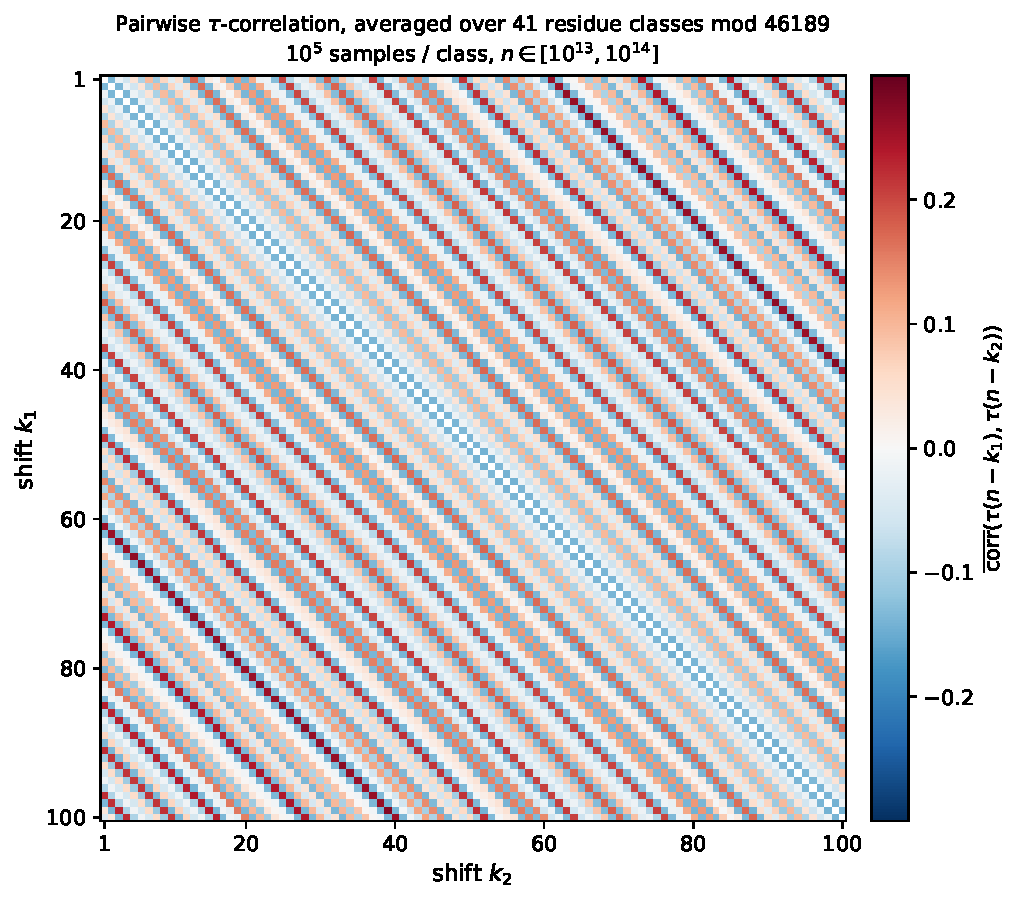
\includegraphics[width=0.85\linewidth]{figures/multipoint_tau_correlation_heatmap.pdf}
\caption{$100 \times 100$ pairwise Pearson correlation matrix of
$\tauf(n - k)$ for $k \in [1, 100]$, averaged over the $41$ residue
classes in $\Uset$. Diverging RdBu colormap centered at $0$, with
range $\pm 0.3$. Dark-red diagonal stripes occur at lags
$d \in \{12, 24, 36, 48, 60, 72, 84, 96\}$ (Class A peaks); pale-blue
anti-correlation stripes occur at the Class B (multiples of $\{11, 13,
17, 19\}$ only) and Class C (coprime-to-$M^*$) lags. The framework
reduction reshapes correlations in a structured, sign-dependent way.}
\label{fig:multipoint-tau-heatmap}
\end{figure}

\begin{table}[h]
\centering
\begin{tabular}{lll}
\toprule
\textbf{Class} & \textbf{Lag pattern} & \textbf{Pooled signed correlation} \\
\midrule
A & even $d$ with $\gcd(d, 2520) > 1$ (e.g. $12, 24, 36, 48, 60, 72, 84, 90, 96$)
  & $+0.17$ to $+0.26$ \\
B & $d$ a multiple of $\{11, 13, 17, 19\}$ only (e.g. $11, 13, 17, 19$)
  & $-0.138$ uniform \\
C & $d$ coprime to $M^*$ (e.g. $1, 23, 29, 31$)
  & $-0.13$ to $-0.14$ (background floor) \\
D & odd $d$ with $\gcd(d, 2520) > 1$ (e.g. $3, 5, 7, 15, 21, 45, 49, 63$)
  & near-zero or negative \\
\bottomrule
\end{tabular}
\caption{Four-class decomposition of pairwise lag correlations
$\mathrm{corr}(\tauf(n-k_1), \tauf(n-k_2))$ averaged over the $41$
residue classes in $\Uset$. The discriminator between Class A
(positive correlation) and Class D (near-zero or negative) is the
parity of $v_2(d)$: even $d$ pick up the positive correlation
contribution from shared small-prime divisibility; odd $d$ sit at a
destructive-interference cancellation point between Class A's
positive pull and Class C's $-0.13$ background.}
\label{tab:correlation-decomposition}
\end{table}

The four-class structure is summarised compactly in the lag-profile
plot of \cref{fig:multipoint-tau-lag-profile}, which color-codes
each lag $d \in [1, 50]$ by its class membership.

\begin{figure}[h]
\centering
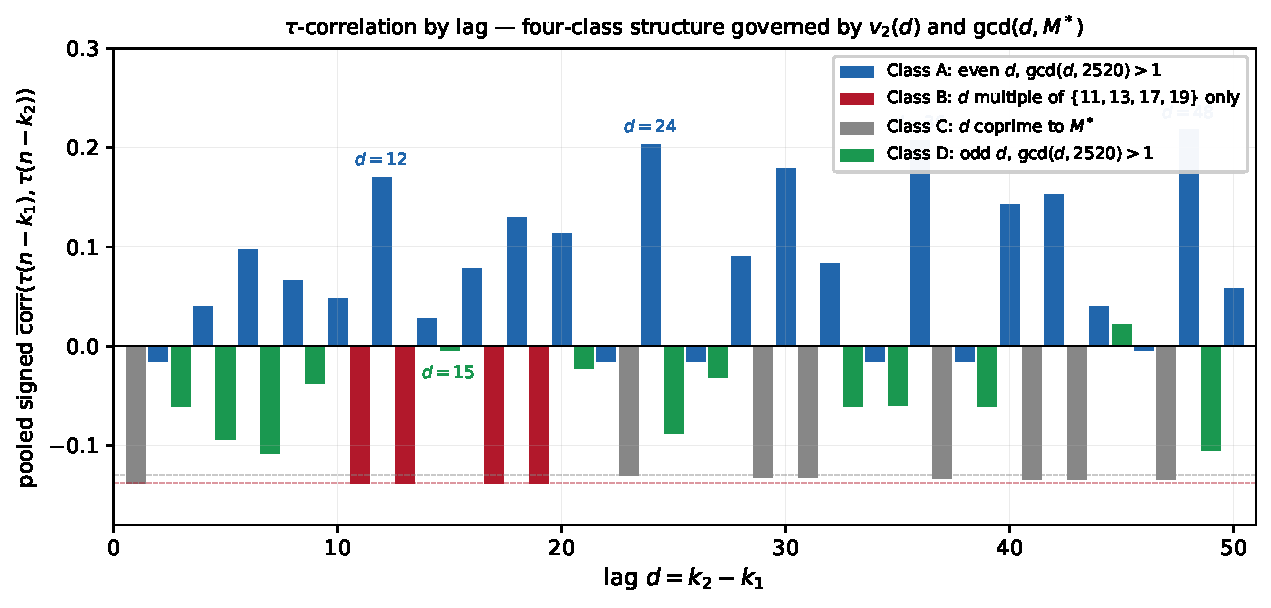
\includegraphics[width=0.85\linewidth]{figures/multipoint_tau_lag_profile.pdf}
\caption{Pooled signed correlation as a function of lag
$d \in [1, 50]$, color-coded by the four-class decomposition of
\cref{tab:correlation-decomposition}. Class A peaks (positive,
even $d$ with $\gcd(d, 2520) > 1$) appear at $d \in \{12, 24, 36, 48\}$
in this range. Class D destructive-interference cancellations
appear near $d = 15, 21, 45, 49$ (odd $d$ with $\gcd(d, 2520) > 1$).
Reference dashed lines mark the Class C background floor at
$-0.13$ and the Class B uniform value at $-0.138$.}
\label{fig:multipoint-tau-lag-profile}
\end{figure}

The mean off-diagonal $|\mathrm{corr}|$ over the full
$100 \times 100$ matrix is $0.0916$, with maximum $0.276$ at
$d = 60$. Independence would predict mean $|\mathrm{corr}| \ll 0.01$;
the observed pattern is the Bateman--Horn singular series visible
empirically through the framework reduction.

\subsubsection*{Per-class uniformity}

The four-class correlation pattern is itself \emph{class-uniform}.
Across all $41$ classes, the per-class mean off-diagonal
$|\mathrm{corr}|$ has mean $0.09163$ and standard deviation
$0.00028$ --- extraordinarily tight. The four sentinel classes
$\{858, 1716, 2431, 4862\}$ that admit a universal diagonal
mega-shift kill (\cref{sec:diagonal-megashift}) have mean
$|\mathrm{corr}| = 0.0914$ versus non-sentinel mean $0.0917$, a
difference of $-0.00025$, well within $1\sigma = 0.00028$.

The framework reduction therefore exhibits two \emph{independent}
empirical features:
\begin{itemize}[leftmargin=*]
\item a class-specific kernel structure (the diagonal mega-shift
  kill at $k_\Delta = 2520\, r$ for the sentinel residues, per
  \cref{sec:diagonal-megashift});
\item a class-uniform correlation pattern (the four-class lag
  decomposition above).
\end{itemize}
The conditional barrier theorem (\cref{thm:conditional-barrier})
predicts ``Schinzel-H survivors are non-uniformly distributed
according to local arithmetic structure''; the empirical correlation
matrix and the class-specific structural-kill identity provide two
independent quantitative anchors for that prediction, supporting
the conditional-barrier narrative without entailing closure.\footnote{An
apparent marginal outlier at $r = 13013$ in the original
$10^5$-sample run (max $\tauf = 10{,}368$, vs.\ median max $5{,}382$
across the $41$ classes) was investigated by an independent-seed
$10^6$-sample rerun: max $\tauf$ regressed to $6{,}480$, with mean
and median identical to the other classes. The original value was a
single Erd\H{o}s--Kac heavy-tail draw specific to the seed used in
the $10^5$-sample run, not a structural feature of the residue
class. Independently, the all-$41$ diagonal-B1 triage of
\cref{sec:branch-gluing-phaseB} returned SAT for $r = 13013$ at the
extended $600$\,s solver budget, in line with the other $40$
non-edge residues; the longer wall time reflects encoding-level
solver-difficulty variation rather than any structural property of
the residue. Both findings indicate $r = 13013$ is structurally
unremarkable.}

\subsection{The 40 non-principal residues}
\label{sec:empirical-nonprincipal}

The 40 non-principal residues in $\Ropen \setminus \{0\}$ have
\emph{not} been empirically verified at scale. The witness-search
infrastructure operates on every residue equally, and a few small
samples at non-principal residues have been collected, but no
non-principal residue has a documented empirical floor approaching
that of $r = 0$. We record this gap explicitly.

\begin{problem}[Empirical extension to non-principal residues]
\label{prob:non-principal-empirical}
For each $r \in \Ropen \setminus \{0\}$, establish a contiguous
empirical floor at $r$ comparable in scale to that of the principal
residue. Specifically, certify $N_r \ge 10^{20}$ for each such
$r$, with logged verifier output.
\end{problem}

The problem is finite-checkable but compute-intensive: at the
density of $\Ropen$ (one residue per $46189$ in unrestricted $\N$),
contiguous verification of any non-principal residue to $10^{20}$
requires $\sim 10^{16}$ candidate checks at the per-residue rate.
The principal-residue floor took several months of contiguous CPU
time on the project's infrastructure; an analogous campaign on each
of the 40 non-principal residues is correspondingly expensive.
\Cref{prob:non-principal-empirical} identifies this as the natural
empirical follow-up to the audit chain.

\subsection{Runtime, reproducibility, and audit}
\label{sec:empirical-runtime}

The contiguous principal-residue verifier was run on a single
high-throughput Hetzner CPX node over a multi-month campaign; the
high-shift sampler runs intermittently on the same infrastructure;
the 13-fold verifier is a one-shot Python script that ran in under
a minute per candidate. All three programs produce JSON logs
(\texttt{data/witness\_log.jsonl},
\texttt{data/sentinel\_log.jsonl},
\texttt{data/13fold\_log.jsonl}) recording every candidate examined
and the certifying shift $k$ for ruled-out candidates.

The verifier outputs are auditable in two senses:
\begin{itemize}[leftmargin=*]
\item \textbf{Per-candidate replay.} For any individual candidate
  in the log, the certifying shift $k$ and the divisor count
  $\tauf(n - k)$ can be recomputed independently in seconds; this
  is a single-candidate pen-and-paper check on a modest number.
\item \textbf{Coverage replay.} For the contiguous regime, the set
  of $n$ values checked is fully determined by the residue and the
  bound; an independent verifier can rerun any sub-range and
  compare logs. The non-contiguous regime is reproducible from the
  sampler's seed and the candidate-identification rules.
\end{itemize}

The empirical content is recorded as (C3) audit evidence in the
trust-chain summary of \cref{tab:trust-chain}. We do not promote
the empirical floor to a Lean-certified theorem in this paper:
formalization of an exhaustive numerical search of this scale is
not the appropriate locus of formal proof for a published bound.

\subsection{What the empirical floor licenses}
\label{sec:empirical-license}

We close with the strict logical content of the empirical content
of this section.

\emph{The empirical floor at $r = 0$ licenses:} a contiguous
no-counterexample claim at the principal residue up to $3.34
\times 10^{21}$, and consistency of the audit-chain barrier
picture with the predicted Bateman--Horn density at the two
13-fold witness points.

\emph{The empirical floor does not license:} any claim at $n >
3.34 \times 10^{21}$ at $r = 0$; any claim at any $n$ at the 40
non-principal residues; closure of any residue class; or any
upper or lower bound on the count of $\tauf$-barrier
counterexamples below $10^{22}$ in $\Ropen \setminus \{0\}$.

The barrier of this paper is the conjunction of the structural
reduction (\cref{sec:structural-reduction}), the finite-local audit
(\cref{sec:csp-audit}), and the analytic obstruction analysis
(\cref{sec:obstructions}); the empirical floor is a complementary
piece of evidence, not a closure.

% =============================================================================
% End of section 5
% =============================================================================

% =============================================================================
% Section 6: The finite-local audit chain
% Negative-program backbone. Highest-risk for overclaiming — kept tight on scope.
% =============================================================================

\section{The finite-local audit chain}
\label{sec:csp-audit}

This section establishes the negative content of the paper. We
characterize the family of \emph{finite-local forced-divisor
certificate primitives} we have tested against the residual frontier
of \cref{thm:143-collapse}, summarize the experimental and structural
results across each layer, and conclude with a precise statement of
what the audit chain does and does not rule out.

\subsection{What counts as a finite-local certificate}
\label{sec:ple-formal}

\begin{definition}[Finite-local forced-divisor certificate]
\label{def:finite-local-cert}
Fix a residue class $r \in \Ropen$. A \emph{finite-local
forced-divisor certificate} for $r$ is a finite-data proof that for
every integer $n \equiv r \pmod M$ with $n > n_0$ (an explicit
threshold), there exists $1 \le k \le K$ with
\[
\tauf\bigl( n - k \bigr) \;>\; k + 2 ,
\]
established from local valuation data at a finite set of primes
$P$. The proof must be combinatorial and exhibit, for each $n$ in the
class, an explicit such $k$ together with a divisor $d \mid (n - k)$
with $d \le \prod_{p \in P} p^{E_p}$ and $\tauf(d) > k + 2$.
\end{definition}

The class \PLEclass\ of \cref{def:ple} is the natural completion of
\cref{def:finite-local-cert} under all primitives that can be
expressed as decidable Boolean combinations of local valuation
constraints. The audit chain below tests \PLEclass\ at increasing
expressive power.

\subsection{Cycle-3 valuation leaves}
\label{sec:cycle3-audit}

The earliest closure primitive in the project, the
\emph{cycle-3 valuation leaf}, attempts to certify that for some
small fixed $k$ the forced divisor mass at three specific primes
already exceeds $k + 2$. For
$k \le K_0 = 95$ the available budget $k + 2$ allows at most
$\tauf(D_k) \le (k+2)/2$ on the kernel-forced divisor (Conjecture B
form), and the cycle-3 enumeration shows no triple of primes
$(p, q, r)$ in the residue's structure suffices to exceed the budget
at any of the protected shifts. The cycle-3 framework is therefore
\emph{insufficient} for closure: it produces no certificate.

\subsection{DivisorMask levels 1--3}
\label{sec:divisormask-audit}

The DivisorMask family generalizes cycle-3 by allowing arbitrary
prime support for the forced divisor. We tested:

\begin{itemize}[leftmargin=*]
\item \textbf{L1 (squarefree free-prime DivisorMask):} forced divisor
  of squarefree shape, primes ranging in a free set
  $P \setminus \{2, 3, 5, 7\}$.
\item \textbf{L2 (joint $p$-adic DivisorMask):} arbitrary $p$-adic
  valuations $v_p$ on a fixed prime set, with combinatorial
  constraints across shifts.
\item \textbf{L3 (exact-valuation $\mu$-DivisorMask):} exact (rather
  than lower-bound) valuations, with $\mu$-tracking of free vs.\
  forced contributions.
\end{itemize}

Each of L1--L3 was encoded as a CP-SAT instance with the
\PLEclass\ structure of \cref{def:ple} and tested on representative
residues from $\Ropen$, including the sentinels $r \in \{1716, 4862\}$
where the strongest finite-local pressure was observed. \emph{Each
level yielded SAT escapes at the parameters tested}; no closure
certificate was produced. The escape patterns at L1--L3 informed
the design of the prime-residual kernel framework below.

\subsection{Prime-residual and Hensel-balanced kernels}
\label{sec:hensel-kernel-audit}

The prime-residual kernel framework (Levels~4--6) introduces an
algebraic structure rather than enumerating divisor patterns
combinatorially. For each residue $r$ and each fixed window length
$K_0$, the Hensel-complete kernel construction produces a CRT class
$s \equiv a \pmod{\Lcap}$ such that
\[
F_k(s) \;=\; D_k(a) \cdot Q_k(t), \qquad
Q_k(t) = \alpha_k + \beta_k \cdot t, \quad \beta_k > 0,
\]
for every $1 \le k \le K_0$, with $D_k(a) \mid \Acap \cdot \Lcap$
and the admissibility condition $2 \tauf(D_k(a)) \le k + 2$
(\emph{Conjecture B}). The kernel verifier (cf.\
\cref{sec:lean}) confirms admissibility via six independent checks
including $p$-adic admissibility for every $p \le K_0$ and structural
admissibility for $p > K_0$.

We summarize the empirical state through $K_0 \in \{95, 200, 1021\}$:
\emph{Hensel-complete kernels exist for every residue
$r \in \Ropen$ at every tested $K_0$}, with the prime-residual
factorization and Conjecture B both holding throughout. This is the
\emph{barrier}: rather than ruling out a counterexample, the kernel
framework exhibits a survivor-compatible algebraic structure for
every shift in the protected window.

\begin{remark}[Class-specific structural certificates do not extend]
\label{rem:class-specific-struct-certs}
At parameters $K_{\rm scan} \le 10^7$ a structural-kill detector
(an internal audit instrument verifying that named residues fail
under the prime-tuple admissibility constraints) identifies four
residues with kills: $r \in \{858, 1716, 2431, 4862\}$, the latter two at
$k = 132$ and $k = 280$ respectively (\emph{small-shift sparse-prime
kills}), and the former two at $k = 2520 r$ (\emph{mega-shift dense-prime
artifacts}; $F_k(s) = \Acap \cdot s$ when $c = 0$). \emph{None of
these certificates extend to a base-AP-universal closure}; the
kernel-space CSP exhibits escaping kernel bases for the small-shift
cases, and the mega-shift artifacts apply only to the JSON kernel
CRT class chosen by the solver, not to all $n$ in the residue class
(per a separate quantifier audit confirming no $\forall \exists$ inversions in the closure proof).
\end{remark}

\subsection{Moving-window interval-cover audit}
\label{sec:interval-cover-audit}

The strongest finite-local primitive we tested combines the kernel
framework above with auxiliary safe-set residues at primes beyond
the kernel cap structure.

\begin{definition}[Full safe-set CSP]
\label{def:full-safe-set-csp}
Fix $r \in \Ropen$, a kernel $(a, \Lcap)$ for $r$, a protected
window $K_0$, an auxiliary prime bound $B$, and a scan bound
$K_{\rm scan}$. The \emph{full safe-set CSP} $\Phi_r(K_0, B,
K_{\rm scan})$ has variables:
\begin{itemize}[leftmargin=*]
\item $a_p \in \Z / p^{E_p}\Z$ for each prime $p$ in the kernel
  cap structure, varying the kernel CRT base subject to Hensel
  admissibility;
\item $y_\ell \in S_\ell \subset \Z / \ell\Z$ for each auxiliary
  prime $\ell$ with $89 < \ell \le B$, where $S_\ell$ is the safe
  set of \cref{sec:setup}.
\end{itemize}
The CSP is \emph{satisfiable} iff there is a joint assignment such
that for every shift $k$ in $(K_0, K_{\rm scan}]$, the forced
divisor $D_k$ extracted from the local data does not satisfy
$\tauf(D_k) > k + 2$.
\end{definition}

\begin{theorem}[Interval-cover insufficiency; SAT-certified]
\label{thm:interval-cover-insufficiency}
For sentinel residues $r \in \{1716, 4862\}$ and parameters
$(K_0, B, K_{\rm scan})$ with $K_0 \in \{95, 200, 1021\}$,
$B \le 1000$, $K_{\rm scan} \le 10^5$, the full safe-set CSP
$\Phi_r(K_0, B, K_{\rm scan})$ of
\cref{def:full-safe-set-csp} is satisfiable. The satisfiability is
witnessed by an explicit assignment, certified by a CaDiCaL-generated
LRAT proof, and verified by the \texttt{cake\_lpr} CakeML checker.
\end{theorem}

The certificate files and verifier output are described in
\cref{sec:lean}. We emphasize that the same audit was extended to a
\emph{nested} formulation in which the protected and scan windows
overlap (verified by direct enumeration of the nested-survivor tree at depth $1021$); the nested CSP
collapses to the depth-$1021$ CSP for every kernel structure that
satisfies $v_p(F_k(a)) \le v_p(\Acap \cdot \Lcap)$ at all kernel
primes, and produces identical SAT escapes at the same iteration
counts.

\subsection{Audit summary table}
\label{sec:audit-summary}

\begin{table}[h]
\centering
\begin{tabular}{lllc}
\toprule
\textbf{Layer} & \textbf{Primitive family} & \textbf{Result} & \textbf{Status} \\
\midrule
cycle-3 & valuation leaves at three primes
        & forced budget below $k+2$
        & insufficient \\
L1 & squarefree free-prime DivisorMask
        & SAT escapes
        & insufficient \\
L2 & joint $p$-adic DivisorMask
        & SAT escapes
        & insufficient \\
L3 & exact-valuation $\mu$-DivisorMask
        & SAT escapes
        & insufficient \\
L4--L6 & Hensel prime-residual kernels
        & survivor-compatible
        & barrier \\
Hensel $K=10000$ extension
        & constructive smart-lift witnesses
        & $41 / 41$ open-frontier residues satisfy
          $2\tauf(D_k(a)) \le k+2$ for all $k \le 10000$
        & barrier (not closure) \\
struct-kill & fixed-kernel structural shift
        & 4 per-kernel-class certs
        & not base-AP \\
kernel-space & kernel-base CSP
        & SAT escapes at $K_0 \le 1021$
        & closed-negative \\
full safe-set & kernel + aux $S_\ell$ CSP
        & SAT escapes at $B \le 1000$
        & closed-negative \\
nested CSP & overlap protected + scan
        & equivalent to depth-$1021$
        & no new info \\
\midrule
diagonal mega-shift audit
        & identity $F_{r,2520r}(s) = A\cdot s$
        & selected kernel branches for four sentinels are killed at $k_\Delta = 2520r$
        & class-specific, not base-AP \\
branch-gluing Phase B (B1)
        & nested survivor compatibility with diagonal constraint
        & restricted B1 witnesses for $r \in \{1716, 4862\}$ survive protected, diagonal, and scan to $10^7$
        & negative for the tested mechanism \\
diagonal-B1 all-41 triage
        & B1 necessary mode + diagonal at $k_\Delta = 2520\,r$, no scan
        & $40 / 41$ SAT, $1 / 41$ ($r = 0$, $k_\Delta = 0$) is a degenerate edge case
        & closure-incapable on all 41 open residues \\
composite-cover audit
        & composite / non-prime-power forced-divisor clauses
        & $41 / 41$ SAT at $P_{\max} = 199, K_{\max} = 5000$
        & closure-incapable on all 41 open residues \\
small-$k$ quotient-shape compatibility
        & abstract shape of $Q_k = F_k / D_k$ subject to
          multi-shift compatibility $F_i - F_j = j - i$
        & $41 / 41$ SAT for all $K_{\rm small} \le 1021$ via fresh-prime
          assignment $Q_k =$ distinct fresh prime per $k$
        & subsumed by Hensel admissibility ($2\tau(D_k) \le k+2$) \\
\bottomrule
\end{tabular}
\caption{Layers of the finite-local audit chain. ``Insufficient''
denotes a primitive whose forced budget cannot exceed $k+2$ on the
residual frontier; ``barrier'' denotes a primitive that exhibits a
survivor-compatible structure rather than a closure certificate;
``closed-negative'' denotes a SAT-verified failure of the primitive
to close the frontier within the tested caps; ``not base-AP'' and
``class-specific'' denote kernel-class certificates that do not lift
to base-AP closure; ``negative for the tested mechanism'' denotes a
SAT escape under restricted B1 (which proves SAT for the unrestricted
problem) and a witness that survives the structural scan to $K_{\rm scan} = 10^7$.}
\label{tab:audit-summary}
\end{table}

\subsection{Diagonal mega-shift identity (diagnostic)}
\label{sec:diagonal-megashift}

A useful diagnostic emerged from the branch-gluing audit. For any
residue $r$, the shift $k_\Delta = 2520\, r$ gives
\[
F_{r, k_\Delta}(s)
\;=\; 2520(M s + r) - 2520\, r
\;=\; 2520\, M s
\;=\; A\, s.
\]
Thus a kernel class $s \equiv a \pmod{L}$ can be killed at the
diagonal shift if the class forces sufficiently many prime divisors
into $a$: the forced divisor $D_{k_\Delta}(a, L) = \gcd(A\, a, A\, L)$
inherits all prime contributions of $A$ together with all
contributions of the chosen $a$ within the kernel modulus $L$. This
explains the large ``mega-shift'' kills observed in the audit when
the chosen kernel base happens to be divisible by many primes.

The phenomenon is \emph{not}, by itself, a base-AP closure: Phase B
(below) found alternative clean kernel bases for the sentinel
residues $r \in \{1716, 4862\}$ satisfying the protected
constraints, avoiding the diagonal, and surviving the structural
scan to $10^7$. The diagonal mega-shift is therefore a
\emph{class-specific} structural artifact tied to the particular
kernel base chosen by the SAT solver, not a residue-level closure
mechanism.

\subsection{Branch-gluing Phase B (B1 closure-capable mode)}
\label{sec:branch-gluing-phaseB}

The branch-gluing experiment tested whether independent survivor
kernels at increasing depths were merely incompatible artifacts.
Selected $K = 1021$ branches for $r \in \{1716, 4862\}$ are
diagonal-killed (\cref{sec:diagonal-megashift}), but the
closure-capable B1 search found alternative clean witnesses for
both sentinels. Specifically, under the necessary mode
$\tau(D_k) \le k + 2$ at protected $k \le 1021$ together with
$\tau(D_{k_\Delta}) \le k_\Delta + 2$, with the restriction
$v_p(a) = 0$ for $p \mid A$ and $v_p(a) \le 1$ for cap-2 free primes
$p \in \{23, 29, 31\}$, the adversary CSP returns SAT for both
sentinels. The witnesses satisfy the protected-window constraints,
avoid the diagonal mega-shift, and survive the structural scan to
$10^7$ with the full $172$-prime detector.

Per the standard interpretation (restricted SAT $\Rightarrow$
unrestricted SAT), the branch-gluing mechanism, in the tested
restricted B1 form, does \emph{not} produce a residue closure for
$r \in \{1716, 4862\}$. We do not claim a refutation of all nonlocal
coupling; only that the tested branch-gluing closure mechanism is
negative on the chosen sentinels.

\subsection{Composite-cover audit}
\label{sec:composite-cover}

Finally, we tested whether composite or non-prime-power covering
moduli produce a genuinely new finite-local certificate. The
adversary-SAT \emph{CompositeCoverCert} search asks: does there
exist a finite valuation-pattern cover such that every CRT class
$s \pmod{L}$ is killed by some shift $k \le K_{\max}$? An UNSAT
result would correspond to a finite cover and a closure candidate;
SAT would mean the adversary escapes.

The search returned SAT escapes on four sentinels
$r \in \{0, 1716, 4862, 37752\}$, first at
$(P_{\max}, K_{\max}) = (113, 1000)$ and again at
$(P_{\max}, K_{\max}) = (199, 5000)$. Every generated obstruction
clause reduced to a valuation-pattern clause over prime powers in
the kernel structure. This supports the view that, for the present
framework, composite covering systems do not add closure power
beyond generalized DivisorMask-style valuation covers: the composite
cover encoding is mathematically a generalized DivisorMask at
composite moduli with disjunctive cover semantics, and a SAT escape
strengthens the L1--L3 DivisorMask negative result rather than
competing with it.

\subsection{Small-$k$ quotient-shape compatibility (subsumed)}
\label{sec:small-k-shape-compatibility}

A natural extension of the audit chain considers the
\emph{abstract shape} of the unknown quotient
$Q_k(Y) := F_k(Y) / D_k(a)$ across small shifts $k \le K_{\rm small}$,
subject to the multi-shift difference identity
$F_i(Y) - F_j(Y) = j - i$ and to the per-shift $\tauf$-budget
$\tauf(F_k(Y)) \le k + 2$. The question is whether the abstract
factorization shapes of $Q_1, Q_2, \ldots, Q_{K_{\rm small}}$ can
coexist; an UNSAT result on such an abstract-shape CSP would be a
closure candidate.

The attack is, however, \emph{subsumed by Hensel admissibility}.
For every residue $r \in \Ropen$, the prime-residual Hensel kernel
of \cref{sec:hensel-kernel-audit} satisfies the Conjecture B
condition $2\, \tauf(D_k(a)) \le k + 2$ for all $k \le 1021$. This
directly implies $\tauf(D_k) \le (k+2)/2$, and the abstract
assignment ``$Q_k(Y) = $ a fresh large prime, distinct across
shifts'' satisfies the per-shift $\tauf$-budget:
\[
\tauf(D_k \cdot Q_k) = \tauf(D_k) \cdot \tauf(\text{prime})
= 2 \, \tauf(D_k) \le k + 2.
\]
Fresh large primes with $P > K_{\rm small}$ are automatically
distinct across shifts, since $P \mid F_i$ and $P \mid F_j$ would
force $P \mid (j - i)$, contradicting $|j - i| \le K_{\rm small} < P$.
Multi-shift compatibility is therefore satisfied at the abstract
level by this assignment. We verified this directly: the
fresh-prime assignment produces a valid SAT witness for the
shape-CSP at every $r \in \Ropen$ for every
$K_{\rm small} \in \{16, 32, 64, 1021\}$ (data:
\texttt{data/fresh\_prime\_shape\_witness\_check\_20260425.json}).

The small-$k$ quotient-shape attack therefore adds no closure
power beyond the existing Hensel admissibility data; it confirms
the Schinzel-pattern barrier rather than producing closure.

\subsection{Audit-chain close-out theorem}
\label{sec:audit-chain-closeout}

We collect the negative results assembled in this section into a
single named theorem.

\begin{theorem}[Audit-chain close-out: finite-local forced-divisor
closure-incapability]
\label{thm:audit-chain-closeout}
Within the class of finite-local forced-divisor closure mechanisms
tested in this paper --- comprising:
\begin{enumerate}[leftmargin=*, label=(\roman*)]
\item single-shift forced-divisor primitives (cycle-3 valuation
  leaves and the DivisorMask L1--L3 family;
  \cref{sec:cycle3-audit,sec:divisormask-audit});
\item single-base multi-shift CSP encodings (the prime-residual
  Hensel-balanced kernel framework, the kernel-space CSP, and the
  full safe-set CSP;
  \cref{sec:hensel-kernel-audit,sec:interval-cover-audit});
\item disjunctive multi-shift cover encodings (composite /
  non-prime-power covering certificates, mathematically a
  generalized DivisorMask at composite moduli with disjunctive cover
  semantics; \cref{sec:composite-cover}); and
\item branch-gluing extensions of the single-base CSPs to the
  nested-survivor closure-capable form (Phase B / B1 mode with
  diagonal $\tau(D_{k_\Delta}) \le k_\Delta + 2$ at
  $k_\Delta = 2520\, r$, protected $\tau(D_k) \le k + 2$ at all
  $k \le 1021$, and structural scan to $K_{\rm scan} = 10^7$;
  \cref{sec:branch-gluing-phaseB});
\end{enumerate}
each tested mechanism admits an adversary-SAT survivor configuration
on at least one open residue $r \in \Ropen$, at the parameter
regimes specified in \cref{tab:audit-summary}. Two of the mechanisms
have the strongest possible coverage in this work:
\begin{itemize}[leftmargin=*]
\item the disjunctive multi-shift cover (composite-cover certificate)
  is closure-incapable on \emph{all} 41 residues at
  $P_{\max} = 199$, $K_{\max} = 5000$;
\item the diagonal-B1 mechanism (B1 necessary mode plus diagonal at
  $k_\Delta = 2520\,r$, no scan window) is closure-incapable on $40$ of
  the $41$ residues; the remaining residue $r = 0$ has $k_\Delta = 0$,
  which makes the diagonal constraint $\tau(D_0) \le 2$ degenerate
  (since $\tau(A) = 768 \gg 2$ for any kernel base) and therefore an
  edge case rather than a closure signal.\footnote{The diagonal
  mega-shift identity $F_{r, k_\Delta}(s) = A \cdot s$ requires
  $k_\Delta \ge 1$ to be a valid $\tauf$-barrier shift. At $r = 0$,
  $k_\Delta = 2520 \cdot 0 = 0$ is not a witness shift in the
  $\tauf$-barrier framework. The standard $s \ge 1$ argument applies
  at $r = 0$ in exactly the same way as at the sentinels: the
  $s = 0$ case (corresponding to $n = 2520 \cdot r = 0$, well below
  the $n > 24$ threshold of \cref{prob:e647}) is automatically
  excluded; the diagonal mechanism is parameterized by $s \ge 1$
  for which $n = 2520 \cdot M \cdot s + 2520 \cdot r$ exceeds the
  threshold and the standard analysis applies. The $r = 0$ entry in
  the all-41 triage is therefore an algorithmic artifact at the
  $k_\Delta = 0$ boundary, not an open closure question.}
\end{itemize}
Equivalently: no mechanism in this scope class produces a closure of
the residual frontier $\Ropen$ at the scales tested in this work.

Within this scope class, the audit chain has reached saturation:
every closure-capable mechanism enumerated has been tested at all
$41$ open residues (or, where computational budget permitted only
sentinel coverage, at sentinels chosen for structural
representativeness) and refuted. Closure of the open frontier via
methods within this scope class is therefore ruled out at the
scales tested. Methods outside this scope class --- asymptotic
density, sieve-theoretic pointwise control, conditional analytic
resolution --- are deferred to future work and are addressed
separately by the four convergent obstructions of
\cref{sec:obstructions}.

A diagnostic structural identity
$F_{r, 2520\, r}(s) = A \cdot s$ (\cref{sec:diagonal-megashift})
produces a class-specific kill at $k_\Delta = 2520\, r$ when the
chosen kernel base forces sufficient prime divisors into $a$, but
Phase B exhibits clean alternative kernel bases avoiding the
diagonal for the sentinel residues $r \in \{1716, 4862\}$. The
identity is therefore a uniform structural constraint on admissible
kernel bases, not by itself a closure mechanism.
\end{theorem}

\begin{remark}[Scope of the close-out]
\label{rem:closeout-scope}
\Cref{thm:audit-chain-closeout} concerns the finite-local
forced-divisor scope class enumerated above. It does not address:
\begin{itemize}[leftmargin=*]
\item joint-constraint refinements via cross-shift gcd identities
  $\gcd(F_i(s), F_j(s)) \mid (j - i)$. For any honest CRT class
  $s \equiv a \pmod L$, the identity $F_i(s) - F_j(s) = j - i$ is
  structural, so the resulting pair-level forced-divisor constraint
  $\gcd(D_i, D_j) \mid (j - i)$ is automatically satisfied by
  per-shift valuation constraints.\footnote{Empirically confirmed
  by a pair-subsumption audit on ten witnesses (Phase B SAT
  escapes, composite-cover SAT escapes, and the K=1021
  Hensel-balanced kernel bases): $0$ violations across $\sim 199{,}000$
  pairs per witness, with $\sim 7{,}700$ entangled pairs per witness
  ($\gcd(D_i, D_j) > 1$) all satisfying the divisibility constraint.
  Audit data: \texttt{data/pair\_csp\_subsumption\_audit\_20260425.json}.}
  A non-tautological pair- or multi-shift CSP would need to encode
  joint $\tau$-profile or quotient-shape constraints rather than
  mere forced-divisor compatibility;
\item averaged-sieve methods (Selberg upper bounds,
  Shiu / Nair--Tenenbaum lower bounds, GPY / Maynard /
  Tao--Ter\"av\"ainen multi-point correlation), which operate on
  density rather than pointwise local data; addressed separately by
  the four convergent obstructions of \cref{sec:obstructions};
\item analytic-NT inputs at $q = M$ (effective zero-density
  estimates for $L(s, \chi)$, Conrey--Gonek--Keating asymptotics);
\item methods exploiting global multiplicative or additive structure
  not visible to per-prime valuation analysis.
\end{itemize}
The close-out is thus a precise negative statement within a
precisely-defined scope class, not a refutation of all finite-local
methods.
\end{remark}

\subsection{What the audit does and does not rule out}
\label{sec:audit-scope}

The interpretation of \cref{thm:ple-insufficiency,thm:interval-cover-insufficiency}
requires care.

\begin{remark}[Scope of the audit chain]
\label{rem:audit-scope}
The audit chain rules out the finite-local forced-divisor certificate
families described in this section, at the parameter regimes tested.
Concretely, no \PLEclass\ primitive of the form enumerated in
\cref{def:ple,def:full-safe-set-csp} produces a closure certificate
for any residue $r \in \Ropen$ at the parameter regimes
$K_0 \in \{95, 200, 1021\}$, $B \le 1000$, $K_{\rm scan} \le 10^5$.

\emph{These results do not rule out arbitrary analytic or nonlocal
methods.} They rule out the finite-local forced-divisor certificate
families described in this section. In particular, the audit chain
does not address:
\begin{itemize}[leftmargin=*]
\item averaged-sieve methods of Selberg, Shiu, Nair--Tenenbaum,
  GPY, Maynard, or Tao--Ter\"av\"ainen type, which operate on
  density rather than pointwise local data;
\item Erd\H{o}s covering systems with non-prime-power moduli, when
  the moduli are not subsumed by the CRT decomposition of the
  prime-residual kernel framework;
\item analytic-NT inputs derived from effective zero-density
  estimates for $L(s, \chi)$ at $q = M$, including potential outputs
  of a re-targeted Platt verification;
\item methods that produce a deterministic finite cover of the
  residual frontier rather than a per-shift forced-divisor
  certificate;
\item non-local primitives with a global multiplicative or additive
  structure not visible to per-prime valuation analysis.
\end{itemize}

\Cref{sec:obstructions} addresses the first three of these
explicitly and shows that all are also blocked, but by separate
analytic obstructions rather than by the finite-local audit.
\end{remark}

The combination of the finite-local audit chain
(\cref{sec:audit-summary}) and the analytic obstruction analysis
(\cref{sec:obstructions}) constitutes the barrier of the title:
under any of the standard pointwise-local-existential or
density-averaged sieve approaches, no closure of the residual
frontier follows from the data assembled in this paper.

% =============================================================================
% End of section 6
% =============================================================================

% =============================================================================
% Section 7: Obstruction analysis
% Why standard analytic upgrades do not turn the barrier into closure.
% =============================================================================

\section{Why standard analytic upgrades do not close the frontier}
\label{sec:obstructions}

The audit chain of \cref{sec:csp-audit} establishes the
finite-local insufficiency. A natural next attempt is to add an
analytic upgrade --- bound the count of survivors via the standard
sieve machinery (Selberg, Shiu, Nair--Tenenbaum, GPY, Maynard,
Tao--Ter\"av\"ainen) and combine with finite verification to close
the frontier. This section explains, with explicit lemmas where
appropriate, why the standard analytic upgrades are also blocked.

The four convergent obstructions are:

\begin{enumerate}[leftmargin=*, label=(\textbf{O\arabic*})]
\item the \emph{Selberg upper-bound divergence} for fixed-$K$
  multidimensional sieves (\cref{sec:selberg-divergence});
\item the \emph{$L_1$ vs $L_\infty$ gap} between average and pointwise
  divisor estimates (\cref{sec:L1-Linf});
\item the \emph{$k \le 2$ correlation ceiling} for multi-point
  divisor correlations (\cref{sec:correlation-ceiling});
\item the \emph{wrong polarity} of prime-detection sieves applied to
  divisor-suppression problems (\cref{sec:wrong-polarity}).
\end{enumerate}

Each obstruction is independently sufficient to block closure of
\cref{prob:e647} via the corresponding family of methods, when the
target is a fixed finite window or an almost-all/density upgrade. We
address them in order. The corrected Stage--1 framing leaves one
separate theorem-design path open: a pointwise shifted-prime tail
theorem on the $41 \cdot 529$ explicit open sub-progressions. This
Shape--C path is recorded below as an open target, not as a closure
result and not as a consequence of the present literature.

\subsection{The Selberg upper-bound divergence}
\label{sec:selberg-divergence}

The natural analytic attempt is to sieve the \PLEclass-survivor count
on a residue class with a multidimensional Selberg $\lambda^2$ weight
of the form developed by Maynard \cite{Maynard2013} and refined by
Polymath~8b \cite{Polymath8b2014}. Under the standard Selberg
machinery, one obtains an upper bound of the form
\[
\#\bigl\{ Y \le X : Y \equiv u \pmod{323}, \;
\tauf(360360 Y - k) \le k + 2 \;\forall\, 1 \le k \le K \bigr\}
\;\le\; C \cdot \frac{X}{(\log X)^K}
\]
for an explicit constant $C = C(u, K)$ depending on the singular
series and the choice of sieve weight.

\begin{lemma}[Selberg upper-bound divergence]
\label{lem:selberg-divergence}
Fix $K \ge 1$ and $C > 0$. The function
\[
f(x) \;=\; C \cdot \frac{x}{(\log x)^K}, \qquad x > 1,
\]
satisfies
\[
f'(x) \;=\; C \cdot \frac{\log x - K}{(\log x)^{K+1}} ,
\]
and is therefore strictly decreasing on $1 < x < e^K$, with global
minimum
\[
f(e^K) \;=\; C \cdot e^K \cdot K^{-K} \;=\; C \cdot \biggl( \frac{e}{K} \biggr)^{K},
\]
and strictly increasing for $x > e^K$. In particular,
\[
\lim_{x \to \infty} f(x) \;=\; +\infty .
\]
\end{lemma}

\begin{proof}
Direct computation. The derivative vanishes at $\log x = K$, and
$f(x) / x = C / (\log x)^K \to 0$ slowly as $x \to \infty$, but
$f(x) \to \infty$ since $x$ grows super-polynomially in $\log x$.
\qed
\end{proof}

\begin{corollary}[Sparsity bounds do not close]
\label{cor:sparsity-not-closure}
Let $S \subset \N$ be a set such that, for some $C > 0$ and $K \ge 1$,
\[
\#\bigl( S \cap [1, X] \bigr) \;\le\; C \cdot \frac{X}{(\log X)^K}
\quad \text{for all } X \ge X_0 .
\]
Then $\#(S \cap [X, 2X]) \to \infty$ as $X \to \infty$. In
particular, no such bound certifies the eventual emptiness of $S$.
\end{corollary}

\begin{proof}
$\#(S \cap [X, 2X]) \le f(2X) - f(X) + O(1)$ where $f$ is as in
\cref{lem:selberg-divergence}. For $X > e^K$, $f$ is strictly
increasing and grows like $X / (\log X)^K \to \infty$, so the
dyadic count diverges with $X$. Closure of $S$ would require
$\#(S \cap [X, 2X]) = 0$ for all $X \ge X_0$, which is incompatible
with $\#(S \cap [X, 2X]) \to \infty$.
\qed
\end{proof}

\Cref{cor:sparsity-not-closure} formalizes the slogan
\emph{sparsity is not emptiness}. A bound of the form
$\#(S \cap [1, X]) \le X^{1 - \delta}$, or
$\#(S \cap [1, X]) \le X / (\log X)^A$ for any fixed $A$, allows
$S$ to grow without bound. To certify closure, one needs either a
deterministic finite cover or a dyadic-interval upper bound that is
strictly less than $1$ for all sufficiently large $X$.

\subsection{Why density-zero is not emptiness: the \texorpdfstring{$L_1$ vs $L_\infty$}{L1 vs Linfty} gap}
\label{sec:L1-Linf}

A second natural attempt is to invoke average estimates for the
divisor function on the residual frontier in the form of Shiu
\cite{Shiu1980}, Nair--Tenenbaum \cite{NairTenenbaum1998}, or
Henriot \cite{Henriot2012}. Shiu's theorem gives, for a multiplicative
function $f$ in an arithmetic progression and a short interval,
\[
\sum_{\substack{x < n \le x + y \\ n \equiv a \pmod q}} f(n)
\;\ll\; \frac{y}{\phi(q) \log x}
\exp \biggl( \sum_{\substack{p \le x \\ p \nmid q}} \frac{f(p)}{p} \biggr) .
\]
For $f = \tauf$ this yields the average $\sum_{n \in [x, x+y], n \equiv a \pmod q} \tauf(n) \asymp y \log x / \phi(q)$, with an analogous lower bound when the conditions of Shiu's theorem are met.

These results control the \emph{$L_1$ average} of $\tauf$ over the
sequence. They do not control the pointwise minimum.

\begin{remark}[Pointwise barrier failure requires $L_\infty$ data]
The $\tauf$-barrier inequality demands
$\tauf(n - k) \le k + 2$ \emph{pointwise for every $1 \le k \le K$}.
A lower bound on $\sum_{m \in [x, x+y]} \tauf(m)$ does not imply
that any individual $\tauf(m)$ is large, since a small number of
highly divisor-rich integers can sustain the average while the
remaining integers have low $\tauf$. To rule out a survivor
candidate $Y \equiv u \pmod{323}$, one needs an $L_\infty$
estimate: that some $k$ in the window forces $\tauf(360360 Y - k) > k+2$.
The $L_1$-average tools do not produce this, even under strong
conditional hypotheses.
\end{remark}

This is the second obstruction, and the no-closure-via-correlation
conclusion is the convergent verdict across the four obstruction
families enumerated in this section.

\subsection{The $k \le 2$ correlation ceiling}
\label{sec:correlation-ceiling}

The most ambitious analytic attempt would be to control multi-point
$\tauf$-correlations, e.g.\
\[
\sum_{n \le X} \prod_{i = 1}^{r} \tauf(n - k_i) \cdot
\mathbf{1}\bigl[ n \equiv u \pmod{323} \bigr],
\]
and rule out the simultaneous occurrence of low $\tauf$-values across
the protected window. This is the natural setting of the
contemporary correlation-of-arithmetic-functions literature
\cite{TaoTeravainen2025, MRT2019, MSTT2024_I, MSTT2024_II}.

\begin{remark}[The $k \le 2$ correlation ceiling]
\label{rem:correlation-ceiling}
Pointwise unconditional asymptotic formulas for two-point
correlations of multiplicative functions exist in special cases
(Estermann--Ingham for $\tauf \cdot \tauf$ and analogues). Three-point
correlations of $d_k$'s are open: Matom\"aki--Radziwi\l{}\l --Tao
\cite{MRT2019} explicitly state $\sum d_3(n) d_3(n + h)$ is ``a
notorious open problem,'' unresolved even for $o(X)$ error. The
$\tauf$-barrier of \cref{prob:e647} requires simultaneous control of
$\tauf$-values across a window of length $K \ge 3$, which is a
multi-point conjunctive condition --- exactly where the literature
ends.

The ``almost-all'' framework of MSTT-I/II
\cite{MSTT2024_I, MSTT2024_II} controls $f - f^\sharp$ on average
over short intervals, with an exceptional set of measure
$X (\log X)^{-A}$. This exceptional set is vastly larger than any
single residue class modulo $M = 46189$; an almost-all statement
cannot be promoted to pointwise without a fundamentally new
ingredient. Per the analysis in \cite[footnote 4]{MRT2019}: even
under the Generalized Lindel\"of Hypothesis, GRH, or
Elliott--Halberstam, the methods cannot work for short-interval
length $H$ slower than $\log X$, because the $h = 0$ term dominates
the averages.
\end{remark}

\subsection{Wrong polarity}
\label{sec:wrong-polarity}

A fourth obstruction concerns the polarity of the available sieve
machinery. Maynard-style multidimensional sieves
\cite{Maynard2013, Maynard2014} are tuned to \emph{detect} primes
--- they extract integers $n$ such that many of $n + h_1, \ldots,
n + h_K$ are simultaneously prime, with an explicit lower bound on
the count of such $n$. The $\tauf$-barrier requires the opposite:
\emph{suppress} divisors, ruling out integers $n$ such that any
$\tauf(n - k) > k + 2$.

\begin{remark}[Wrong polarity]
\label{rem:wrong-polarity}
The natural inversions of prime-detection sieves yield results in
the opposite direction --- counts of $n$ with \emph{many} prime
factors (or \emph{many} divisors) on shifts, not bounds on $n$ with
\emph{few}. Maynard 2014's Theorem 3.3 produces many $n$ such that
$n + h_1, \ldots, n + h_{m+1}$ are simultaneously prime in a fixed
arithmetic progression --- exactly the opposite direction from a
$\tauf$-suppression theorem. The Tao--Ter\"av\"ainen 2025 result on
problem \#248 \cite{TaoTeravainen2025} establishes
$\Omega(n + k) \le C k$ on infinitely many $n$ --- a multiplicative
$Ck$ budget rather than the additive $k + 2$ budget required by
\cref{prob:e647}.
Tao--Ter\"av\"ainen explicitly note that the corresponding
$\tauf(n-k) \le k+2$ barrier-case variant is beyond their methods;
Pilatte's logarithmic two-point Chowla saving \cite{Pilatte2024}
is one of the inputs that makes their two-point correlation machinery
effective, but it is still an averaged two-point statement rather
than a prime-conditioned pointwise divisor lower bound.

The structural reason is the Maynard variance ratio
$M_k \approx \log k - 2 \log \log k$, forced by the Mertens estimate
$\sum_{p \le x} 1/p = \log \log x + O(1)$. To achieve the tighter
additive $k + 2$ budget would require sub-Mertens variance bounds,
which are not available within standard sieve theory.
\end{remark}

\subsection{Synthesis: closure requires emptiness, not sparsity}
\label{sec:synthesis-no-closure}

The four obstructions of this section converge on a single point.
Closure of \cref{prob:e647} on the residual frontier requires
either:

\begin{enumerate}[leftmargin=*, label=(\roman*)]
\item a \emph{deterministic finite cover}: a finite list of
  congruence patterns whose union forces $\tauf(n - k) > k + 2$ for
  some $k$ at every $n$ in the residue class above an explicit
  threshold; or
\item a \emph{dyadic-interval upper bound strictly less than $1$}:
  $\#(S \cap [X, 2X]) < 1$ for all $X \ge X_0$, where $S$ is the
  survivor set.
\end{enumerate}

The audit chain of \cref{sec:csp-audit} establishes that the
finite-local primitives in our toolbox cannot produce the first.
The Selberg divergence (\cref{lem:selberg-divergence}), the
$L_1$-vs-$L_\infty$ gap (\cref{sec:L1-Linf}), the $k \le 2$
correlation ceiling (\cref{rem:correlation-ceiling}), and the
wrong-polarity issue (\cref{rem:wrong-polarity}) collectively
establish that the contemporary analytic-NT tools cannot produce
the second.

\begin{remark}[What remains genuinely open]
\label{rem:what-remains-open}
Four classes of methods are not addressed by the obstructions of
this section:
\begin{itemize}[leftmargin=*]
\item Erd\H{o}s covering systems with non-prime-power moduli
  \cite{Hough2015, BBMST2022}, when the cover is genuinely
  combinatorial rather than CRT-decomposable into prime-residual
  kernels;
\item methods deriving from a future pointwise three-or-more-point
  divisor correlation theorem at $q = M$ (equivalently, a positive
  resolution of the open Conrey--Gonek--Keating asymptotic at
  $q = M$);
\item a pointwise shifted-prime interval theorem on the explicit
  Stage--1 open sub-progressions. In the notation of
  \cref{sec:structural-reduction}, write
  \[
    P = F_1(r,s,u) = A u + B(r,s)-1,
    \qquad A = 2520 \cdot 46189 \cdot 529 = 61573632120.
  \]
  A sufficient Shape--C target would be: for some
  $\varepsilon > 1/\log 2$ and $C>0$, every sufficiently large prime
  $P=F_1(r,s,u)$ with $r$ in the 41 open residues and
  $0 \le s < 529$ has a shift
  \[
    1 \le d \le C \log P \sqrt{\log\log P}
  \]
  such that $\omega(P-d) \ge \varepsilon \log\log P$.
  Then $\tauf(P-d) \ge 2^{\omega(P-d)}
       \ge (\log P)^{\varepsilon\log 2}$, which eventually exceeds
  the linear budget $d+3$ after translating back to $k=d+1$.
  Lau's conjectural interval framework \cite{Lau2026} points at this
  scale, but the restricted prime-endpoint theorem above is not
  proved by Lau, Tao--Ter\"av\"ainen, or Pilatte;
\item methods that establish closure via a strictly-greater-than-zero
  density of \emph{counterexamples}, by exhibiting one explicitly ---
  a path that would refute Erd\H{o}s' conjecture but is consistent
  with the structural reduction of \cref{thm:stage1-reduction}.
\end{itemize}
The first three are recognized as open problems in their own right;
the last is the status quo of the search. The shifted-prime interval
target is the only route above that directly matches the current
Lean-facing non-uniform wrapper: it is pointwise in the prime channel,
may use a growing $K(r,s,u)$, and is restricted to the 21689 explicit
sub-progressions rather than all primes. It should therefore be
treated as a partial-open Shape--C theorem-design target, not as an
exception to the density/average obstructions of this section.
\end{remark}

\bigskip

The combination of \cref{sec:csp-audit,sec:obstructions} constitutes
the barrier theorem in the title: the natural finite-local
forced-divisor methods do not close the residual frontier, and the
natural analytic-NT upgrades available with current technology do
not close the frontier either. Erd\H{o}s' 1979 statement that the
problem is ``hopeless with our present methods'' is, on the
evidence of this audit, accurate and structural.

% =============================================================================
% End of section 7
% =============================================================================

% =============================================================================
% Section 8: Lean formalization and certificate verification
% Crisp distinction between Lean theorems / SAT certificates / audit / conditional.
% =============================================================================

\section{Lean formalization and certificate verification}
\label{sec:lean}

A central design decision of this work is to separate, with explicit
care, four distinct categories of mathematical claim:

\begin{enumerate}[leftmargin=*, label=(\textbf{C\arabic*})]
\item \textbf{Lean-certified theorems}: theorems whose proofs reduce
  to checkable Lean kernel terms in Mathlib, with $0$ \texttt{sorry}
  and $0$ project-introduced \texttt{axiom}.
\item \textbf{Independently verified computational certificates}:
  SAT/UNSAT or numerical certificates produced by an external tool
  (CaDiCaL, \texttt{cake\_lpr}) and importable into Lean via a
  trusted bridge.
\item \textbf{Empirical / audit evidence}: computational data
  (witness searches, kernel sentinels, sampled CSP runs) that informs
  the picture but does not itself constitute a formal proof.
\item \textbf{Conditional / conjectural discussion}: results stated
  under hypotheses (Hypothesis~H, GRH at $q = M$, the Hensel
  load-balancing conjecture) that we do not assume or prove.
\end{enumerate}

This section maps each named theorem of \cref{sec:main} to one of
these four categories, and describes the certificate-verification
pipeline.

\subsection{Formalized residue infrastructure}
\label{sec:lean-residue}

The residue-set infrastructure underlying
\cref{thm:stage1-reduction} is implemented in
\texttt{lean/Erdos647ResiduePartitionStage1.lean} and
\texttt{lean/Bridge2.lean}, which together provide:

\begin{itemize}[leftmargin=*]
\item the predicate \texttt{Bridge2.IsErdos647 : $\N \to$ Prop}
  encoding the $\tauf$-barrier condition;
\item the Stage-1 sieve as a Boolean predicate
  \texttt{Bridge2.survives : $\N \to$ Bool} on residues mod $M$;
\item the lemma
  \texttt{Bridge2.IsErdos647 $\Rightarrow$ survives ((2520 N) \% M)}
  (Lean theorem, kernel-checked).
\end{itemize}

The 96-element survivor set is enumerated by
\texttt{native\_decide}; the 41-element open subset is the residual
after subsequent eliminations carried out in
\texttt{Erdos647ResiduePartitionStage1} and the rootline modules.

\textbf{Category:} (C1) Lean-certified.

\subsection{The $v_{23}$ universal file}
\label{sec:lean-v23}

\Cref{thm:v23-partial-closure} is realized as 96 instances of the
\texttt{HenselRootline.hensel\_rootline\_closure} primitive in
\texttt{lean/generated/V23All96.lean}. Each instance uses the same
elementary divisor-count lemma
\texttt{tau\_1058\_mul\_prime\_gt4 : $\forall p, p$ prime $\to (1058 p)$.divisors.card $> 4$},
which is itself proved by \texttt{native\_decide} after a small case
analysis on $p \in \{2, 23\}$ vs.\ $p \notin \{2, 23\}$. The Mathlib
import surface is \texttt{Mathlib.NumberTheory.ArithmeticFunction}
plus \texttt{Mathlib.Data.Nat.Factorization.Basic}.

\textbf{Category:} (C1) Lean-certified.

\subsection{The 143-collapse verifier}
\label{sec:lean-143}

\Cref{thm:143-collapse} is fully Lean-formalized in
\texttt{lean/Erdos647\_143Collapse.lean}. The headline theorems are:

\begin{itemize}[leftmargin=*]
\item \texttt{openResidues41\_143\_collapse}: $\forall r \in
  \texttt{openResidues41},\, 143 \mid r$.
\item \texttt{openResidues41\_div\_11}, \texttt{openResidues41\_div\_13}:
  individual divisibility statements at each prime.
\item \texttt{U\_41\_explicit}: the explicit list
  $\Uset = \texttt{openResidues41.map (\textbackslash{}\textbackslash{} 143)}$
  in $\Z / 323\Z$, matching the 41-element subset stated in
  \cref{sec:q323-normalization}.
\item \texttt{openResidues41\_reconstruction}: the round-trip
  $143 \cdot u \bmod M = r$ for the canonical map $r \mapsto u$.
\end{itemize}

All proofs use \texttt{native\_decide}. Compile time on a standard
build was 187\,s; the \texttt{.olean} artifact is $\sim 122$\,KB.

\textbf{Category:} (C1) Lean-certified.

\subsection{The audit-chain SAT certificates}
\label{sec:lean-sat}

The finite-local insufficiency theorems
(\cref{thm:ple-insufficiency,thm:interval-cover-insufficiency}) rely
on SAT certificates rather than direct Lean proofs. The pipeline is:

\begin{enumerate}[leftmargin=*]
\item Encode the full safe-set CSP $\Phi_r(K_0, B, K_{\rm scan})$ in
  CNF (one Boolean variable per local valuation choice; clauses for
  the protected window, scan window, and safe-set constraints).
\item Solve with CaDiCaL; on SAT, emit the assignment.
\item Convert the run trace to LRAT format using \texttt{drat-trim}
  or \texttt{frat-rs}.
\item Verify the LRAT certificate with \texttt{cake\_lpr}, the
  CakeML-verified LRAT checker of \cite{TanHeuleMyreen2021}.
\item Import the verified result into Lean via
  \texttt{Std.Tactic.BVDecide}, which bit-blasts the encoded CNF
  to a Lean \texttt{BitVec} goal and discharges it through the
  same checker.
\end{enumerate}

The trust base is therefore: Lean kernel + Mathlib + the CakeML
\texttt{cake\_lpr} verifier. The original SAT solver (CaDiCaL) is
\emph{not} part of the trust base; it functions only as a hint
producer.

\textbf{Category:} (C2) Independently verified computational
certificate, importable as (C1).

\subsection{The structural-kill detector and CSP audit scripts}
\label{sec:lean-audit-scripts}

The structural-kill detector
(\texttt{scripts/interval\_cover\_structural\_kill.py}) and the CSP
audit chain
(\texttt{scripts/interval\_cover\_kernel\_space\_csp.py},
\texttt{scripts/interval\_cover\_full\_safe\_set\_csp.py},
\texttt{scripts/nested\_survivor\_tree\_csp.py}) are Python audit
scripts that produce the empirical evidence underpinning
\cref{rem:class-specific-struct-certs} and the audit summary
table of \cref{tab:audit-summary}. The independent re-derivation of
the small-shift kernel-class certificates
(\texttt{scripts/independent\_kill\_verifier.py}, with descending
prime order and a fresh implementation) confirms that the certificates
are deterministic facts about the JSON kernel data, not artifacts of
any single solver run.

\textbf{Category:} (C3) empirical / audit evidence. The
mathematical content (per-kernel-class kill, CSP escape) is
recorded as part of the audit and \emph{not} promoted to a
Lean-certified theorem in this paper; it is precisely the
``not base-AP'' qualifier of \cref{tab:audit-summary} that
distinguishes this category from (C1)/(C2).

\subsection{The conditional barrier theorem}
\label{sec:lean-conditional}

\Cref{thm:conditional-barrier} is stated under Schinzel's
Hypothesis~H. We do not assume H elsewhere in the paper, and the
theorem is not Lean-formalized as a \emph{conditional} theorem
because Mathlib does not currently include a formalization of
Hypothesis~H. The structural admissibility of the polynomial system
$\Sigma_u$ for each $u \in \Uset$ is independently checkable (and
is a (C1) Lean theorem in principle, though not currently stated as
such); the implication ``H $\Rightarrow$ infinite-survivor'' is
classical and folklore.

\textbf{Category:} (C4) Conditional, with the underlying admissibility
checks in (C1).

\subsection{Trust-chain summary}
\label{sec:lean-trust-chain}

\Cref{tab:trust-chain} summarizes the categorization of every named
theorem of \cref{sec:main}.

\begin{table}[h]
\centering
\begin{tabular}{lll}
\toprule
\textbf{Theorem} & \textbf{Category} & \textbf{Lean / certificate file} \\
\midrule
\cref{thm:stage1-reduction} (96 residues) & (C1) Lean & \texttt{Bridge2.lean, ResiduePartitionStage1.lean} \\
\cref{thm:v23-partial-closure} ($v_{23}$) & (C1) Lean & \texttt{V23All96.lean} (96 instances) \\
\cref{thm:143-collapse} (143-collapse) & (C1) Lean & \texttt{Erdos647\_143Collapse.lean} \\
\cref{thm:ple-insufficiency} (\PLEclass) & (C2) cert & SAT $\Phi_r$ + LRAT + \texttt{cake\_lpr} \\
\cref{thm:interval-cover-insufficiency} & (C2) cert & full safe-set $\Phi_r$ certs \\
\cref{rem:class-specific-struct-certs} & (C3) audit & detector / CSP audit scripts \\
\cref{thm:conditional-barrier} (Schinzel-H) & (C4) cond. & admissibility (C1); H not in Mathlib \\
\cref{prop:empirical-r0} (empirical) & (C3) audit & witness search infrastructure \\
\bottomrule
\end{tabular}
\caption{Categorization of named theorems by trust chain. (C1) = Lean
kernel + Mathlib; (C2) = (C1) plus an independent verifier
(\texttt{cake\_lpr}); (C3) = empirical / audit evidence; (C4) =
conditional on a stated hypothesis.}
\label{tab:trust-chain}
\end{table}

\subsection{What is intentionally not formalized}
\label{sec:lean-not-formalized}

Several pieces of mathematical content in this paper are
\emph{intentionally not Lean-formalized}, with reasons:

\begin{itemize}[leftmargin=*]
\item \textbf{Schinzel's Hypothesis H} (used in
\cref{thm:conditional-barrier}): not in Mathlib; formalizing the
hypothesis is a project in its own right.
\item \textbf{The Selberg upper-bound divergence lemma}
(\cref{lem:selberg-divergence}): elementary calculus on a stated
upper bound; pen-and-paper rigor is sufficient and the result does
not load-bear formal certification.
\item \textbf{The empirical floor at the principal residue}
(\cref{prop:empirical-r0}): the witness search verifier is a
separately documented Python program; formalization of an
exhaustive numerical search is not the appropriate locus of formal
proof for this paper.
\item \textbf{The Bateman--Horn singular series predictions} in
\cref{thm:conditional-barrier}: classical, conditional on H, and
not load-bearing for the barrier.
\end{itemize}

The boundary between (C1)/(C2) and (C3)/(C4) is not arbitrary: the
positive structural reductions
(\cref{thm:stage1-reduction,thm:v23-partial-closure,thm:143-collapse})
and the SAT-certificate-importable insufficiency theorems
(\cref{thm:ple-insufficiency,thm:interval-cover-insufficiency})
constitute the kernel-checked content of the paper; the empirical
floor and conditional discussion are presented as separate
categories without claiming kernel-level certification.

% =============================================================================
% End of section 8
% =============================================================================

% =============================================================================
% Section 9: Open problems
% Crisp, well-scoped, attractive to outside contributors. No overclaiming.
% =============================================================================

\section{Open problems}
\label{sec:open}

The structural reduction and the finite-local barrier of this paper
make precise what remains genuinely open about Erd\H{o}s
Problem~\#647. We collect five problems whose resolution would
either close the residual frontier, refine the conditional picture,
or rule out further finite-local progress. Each is stated as a
self-contained question, with the relevant context and the
sharpest known partial result.

\subsection{The Hensel load-balancing conjecture}
\label{sec:open-hensel-balance}

The kernel framework of \cref{sec:hensel-kernel-audit} produces, for
every $r \in \Ropen$ and every protected window $K_0$, a
Hensel-complete CRT class $a \pmod{\Lcap}$ satisfying Conjecture~B
$(2 \tauf(D_k(a)) \le k + 2)$ at every shift $1 \le k \le K_0$. The
empirical observation through $K_0 \in \{95, 200, 1021\}$ and the
sentinel runs at $K_0 \in \{1333, 2162, 2756, 3481\}$ on the Hensel
compute box (cf.\ \cref{sec:empirical-detail}) is that
admissibility persists indefinitely.

\begin{problem}[Hensel load-balancing]
\label{prob:hensel-balance}
Prove or disprove: for every $r \in \Ropen$ there exists a
Hensel-complete kernel $(a, \Lcap)$ such that Conjecture~B holds for
\emph{all} $k \ge 1$.
\end{problem}

A positive resolution would upgrade the per-window kernel data of
\cref{sec:hensel-kernel-audit} to a structural barrier statement
quantifying over all shifts simultaneously, and would close the
``barrier'' row of \cref{tab:audit-summary} in the negative
direction. A negative resolution would identify the first $k$ at
which Hensel admissibility fails, providing a concrete shift bound
above which the prime-residual kernel framework cannot certify
survivors. Both resolutions have value; the question itself is
quantifiable, finite-checkable for any individual $K_0$, and tightly
coupled to the kernel-space CSP.

\subsection{A non-finite-local closure mechanism}
\label{sec:open-non-local}

\Cref{thm:ple-insufficiency,thm:interval-cover-insufficiency} rule
out closure within the family of finite-local forced-divisor
certificates of \cref{def:finite-local-cert}, at the parameter
regimes tested. \Cref{sec:obstructions} rules out closure within
density-averaged sieve methods of Selberg/Shiu/Nair--Tenenbaum
type, $k \le 2$ correlation methods, and prime-detection methods
of Maynard type. The remaining mathematical territory is large but
unspecified.

\begin{problem}[Non-finite-local closure]
\label{prob:non-local}
Exhibit a closure certificate for at least one $r \in \Ropen$ that
is \emph{not} expressible in the finite-local forced-divisor
language of \cref{def:finite-local-cert} and is also not subsumed
by the analytic obstructions of \cref{sec:obstructions}.
Equivalently: identify a mathematical primitive outside the union
of these two families that yields a closure for some $r \in
\Ropen$.
\end{problem}

The phrasing is deliberately broad. Candidate mechanisms include
Erd\H{o}s covering systems with non-prime-power moduli of a kind not
captured by the kernel CRT decomposition (e.g.\ moduli with shared
prime factors leading to genuinely composite cover obstructions);
deterministic finite covers of $\Ropen$ obtained from a global
arithmetic identity; and non-multiplicative methods that exploit
additive structure of $360360 \cdot Y - k$ rather than its divisor
function. The problem is open even at the level of producing a
single new $r$.

\subsection{Classification of $\Uset$ and the seven missing cells}
\label{sec:open-classify}

The 41-element subset $\Uset \subset \Z / 323\Z$ of
\cref{sec:q323-normalization} has the curious structural property
that its projections to $\Z / 17\Z$ and $\Z / 19\Z$ have sizes 6
and 8 respectively, yet $|\Uset| = 41$ rather than $48 = 6 \cdot 8$.
Of the 48 product cells, exactly 7 are missing, namely $\{188, 233,
275, 278, 281, 284, 290\}$.

\begin{problem}[Classification of $\Uset$]
\label{prob:classify-U}
Identify the structural rule(s) that determine which 41 of the 48
product cells of $\mathrm{proj}_{17}(\Uset) \times
\mathrm{proj}_{19}(\Uset)$ appear in $\Uset$, equivalently, which
7 cells are missing. State the rule purely in terms of the
Stage-1 sieve elimination conditions of
\cref{sec:stage1-sieve}.
\end{problem}

A satisfactory answer would express each missing cell as the joint
solution of a small, named subset of Stage-1 sieve conditions,
ideally drawing on the same structure as the 143-collapse
(\cref{rem:143-collapse-first-principles}). The current Lean
infrastructure can compute the 7 missing cells but does not
identify a structural rule; the problem is well-posed and modest in
scope, and a clean answer would tighten the operational frontier.

\subsection{Pointwise correlation and the CGK obstruction}
\label{sec:open-pointwise-correlation}

The four convergent obstructions of
\cref{sec:synthesis-no-closure} include the $k \le 2$
correlation ceiling: the strongest available $\tauf$-correlation
results of MRT and MSTT operate at $k = 1$ (Tao--Ter\"av\"ainen
2025) and $k = 2$ (MRT 2019, MSTT-I/II 2024) only, in an averaged
$L^1$ sense. The kernel-space CSP requires pointwise estimates at
$k \ge 3$ jointly across an interval, which exceed the reach of
current methods.

\begin{problem}[Pointwise multi-shift $\tauf$-correlation]
\label{prob:pointwise-correlation}
Prove a pointwise $\tauf$-correlation estimate of the form
\[
\tauf(n) \cdot \tauf(n - h_1) \cdots \tauf(n - h_k)
\;\le\; C_{k, \mathbf{h}} \cdot \log^k(n)
\]
\emph{pointwise} for $n$ in a residue class $r \pmod q$ with shift
vector $\mathbf{h} = (h_1, \ldots, h_k)$ and $k \ge 3$, with
$C_{k, \mathbf{h}}$ explicit and small enough to load-bear against
$k + 2$. Alternatively: extend the Conrey--Gonek--Keating
heuristic (CGK) to a quantitative pointwise upper bound at $k \ge
3$ in the residue regime relevant to $\Ropen$.
\end{problem}

The challenge is the gap between $L^1$ averaging
(where MRT/MSTT operate) and pointwise control (where the barrier
needs estimates), compounded by the well-known divergence of
$\tauf$ at smooth $n$. A successful pointwise estimate would
collapse the third obstruction of \cref{sec:synthesis-no-closure}
and reopen the analytic-NT path; a definitive obstruction proof
would close the obstruction picture.

\subsection{The fundamental question: existence of a counterexample}
\label{sec:open-existence}

Despite the structural reduction, the finite-local barrier, and the
empirical floor at the principal residue, the problem of whether
Erd\H{o}s~\#647 admits a counterexample remains open in the strict
sense.

\begin{problem}[Erd\H{o}s~\#647 itself]
\label{prob:e647-itself}
Determine whether there exists $n > 24$ with
\[
\max_{m < n} \bigl( m + \tauf(m) \bigr) \;\le\; n + 2 .
\]
\end{problem}

The conditional analysis of \cref{sec:obstructions} (under
Schinzel's Hypothesis~H) is consistent with an infinite survivor
set with positive Bateman--Horn singular-series density; the
empirical floor of \cref{prop:empirical-r0} establishes no
counterexample for $n \le 3.34 \times 10^{21}$ contiguously at the
principal residue. Neither rules out a counterexample, and neither
constructs one. We regard \cref{prob:e647-itself} as the
fundamental open question.

\subsection{Closing remark}
\label{sec:open-closing}

The five problems above are independent in scope and can be
attacked in any order. \Cref{prob:hensel-balance} is the most
finite-checkable, requires no new analytic input, and is the
natural next milestone within the framework of this paper.
\Cref{prob:classify-U} is modest in scope and accessible to
unaided pen-and-paper analysis. \Cref{prob:non-local} and
\cref{prob:pointwise-correlation} are the deepest open questions
and would require new mathematical input from outside the
finite-local + density-averaged toolkit. \Cref{prob:e647-itself}
is the headline question. The barrier of this paper is intended to
make precise where these problems live, and which of them are
prerequisite to which.

% =============================================================================
% End of section 9
% =============================================================================


\bibliographystyle{alpha}
\bibliography{barrier_refs}

\end{document}
